% Options for packages loaded elsewhere
\PassOptionsToPackage{unicode}{hyperref}
\PassOptionsToPackage{hyphens}{url}
%
\documentclass[
]{article}
\usepackage{lmodern}
\usepackage{amssymb,amsmath}
\usepackage{ifxetex,ifluatex}
\ifnum 0\ifxetex 1\fi\ifluatex 1\fi=0 % if pdftex
  \usepackage[T1]{fontenc}
  \usepackage[utf8]{inputenc}
  \usepackage{textcomp} % provide euro and other symbols
\else % if luatex or xetex
  \usepackage{unicode-math}
  \defaultfontfeatures{Scale=MatchLowercase}
  \defaultfontfeatures[\rmfamily]{Ligatures=TeX,Scale=1}
\fi
% Use upquote if available, for straight quotes in verbatim environments
\IfFileExists{upquote.sty}{\usepackage{upquote}}{}
\IfFileExists{microtype.sty}{% use microtype if available
  \usepackage[]{microtype}
  \UseMicrotypeSet[protrusion]{basicmath} % disable protrusion for tt fonts
}{}
\makeatletter
\@ifundefined{KOMAClassName}{% if non-KOMA class
  \IfFileExists{parskip.sty}{%
    \usepackage{parskip}
  }{% else
    \setlength{\parindent}{0pt}
    \setlength{\parskip}{6pt plus 2pt minus 1pt}}
}{% if KOMA class
  \KOMAoptions{parskip=half}}
\makeatother
\usepackage{xcolor}
\IfFileExists{xurl.sty}{\usepackage{xurl}}{} % add URL line breaks if available
\IfFileExists{bookmark.sty}{\usepackage{bookmark}}{\usepackage{hyperref}}
\hypersetup{
  pdftitle={2016 Election Analysis},
  pdfauthor={Ian Bogley},
  hidelinks,
  pdfcreator={LaTeX via pandoc}}
\urlstyle{same} % disable monospaced font for URLs
\usepackage[margin=1in]{geometry}
\usepackage{color}
\usepackage{fancyvrb}
\newcommand{\VerbBar}{|}
\newcommand{\VERB}{\Verb[commandchars=\\\{\}]}
\DefineVerbatimEnvironment{Highlighting}{Verbatim}{commandchars=\\\{\}}
% Add ',fontsize=\small' for more characters per line
\usepackage{framed}
\definecolor{shadecolor}{RGB}{248,248,248}
\newenvironment{Shaded}{\begin{snugshade}}{\end{snugshade}}
\newcommand{\AlertTok}[1]{\textcolor[rgb]{0.94,0.16,0.16}{#1}}
\newcommand{\AnnotationTok}[1]{\textcolor[rgb]{0.56,0.35,0.01}{\textbf{\textit{#1}}}}
\newcommand{\AttributeTok}[1]{\textcolor[rgb]{0.77,0.63,0.00}{#1}}
\newcommand{\BaseNTok}[1]{\textcolor[rgb]{0.00,0.00,0.81}{#1}}
\newcommand{\BuiltInTok}[1]{#1}
\newcommand{\CharTok}[1]{\textcolor[rgb]{0.31,0.60,0.02}{#1}}
\newcommand{\CommentTok}[1]{\textcolor[rgb]{0.56,0.35,0.01}{\textit{#1}}}
\newcommand{\CommentVarTok}[1]{\textcolor[rgb]{0.56,0.35,0.01}{\textbf{\textit{#1}}}}
\newcommand{\ConstantTok}[1]{\textcolor[rgb]{0.00,0.00,0.00}{#1}}
\newcommand{\ControlFlowTok}[1]{\textcolor[rgb]{0.13,0.29,0.53}{\textbf{#1}}}
\newcommand{\DataTypeTok}[1]{\textcolor[rgb]{0.13,0.29,0.53}{#1}}
\newcommand{\DecValTok}[1]{\textcolor[rgb]{0.00,0.00,0.81}{#1}}
\newcommand{\DocumentationTok}[1]{\textcolor[rgb]{0.56,0.35,0.01}{\textbf{\textit{#1}}}}
\newcommand{\ErrorTok}[1]{\textcolor[rgb]{0.64,0.00,0.00}{\textbf{#1}}}
\newcommand{\ExtensionTok}[1]{#1}
\newcommand{\FloatTok}[1]{\textcolor[rgb]{0.00,0.00,0.81}{#1}}
\newcommand{\FunctionTok}[1]{\textcolor[rgb]{0.00,0.00,0.00}{#1}}
\newcommand{\ImportTok}[1]{#1}
\newcommand{\InformationTok}[1]{\textcolor[rgb]{0.56,0.35,0.01}{\textbf{\textit{#1}}}}
\newcommand{\KeywordTok}[1]{\textcolor[rgb]{0.13,0.29,0.53}{\textbf{#1}}}
\newcommand{\NormalTok}[1]{#1}
\newcommand{\OperatorTok}[1]{\textcolor[rgb]{0.81,0.36,0.00}{\textbf{#1}}}
\newcommand{\OtherTok}[1]{\textcolor[rgb]{0.56,0.35,0.01}{#1}}
\newcommand{\PreprocessorTok}[1]{\textcolor[rgb]{0.56,0.35,0.01}{\textit{#1}}}
\newcommand{\RegionMarkerTok}[1]{#1}
\newcommand{\SpecialCharTok}[1]{\textcolor[rgb]{0.00,0.00,0.00}{#1}}
\newcommand{\SpecialStringTok}[1]{\textcolor[rgb]{0.31,0.60,0.02}{#1}}
\newcommand{\StringTok}[1]{\textcolor[rgb]{0.31,0.60,0.02}{#1}}
\newcommand{\VariableTok}[1]{\textcolor[rgb]{0.00,0.00,0.00}{#1}}
\newcommand{\VerbatimStringTok}[1]{\textcolor[rgb]{0.31,0.60,0.02}{#1}}
\newcommand{\WarningTok}[1]{\textcolor[rgb]{0.56,0.35,0.01}{\textbf{\textit{#1}}}}
\usepackage{graphicx,grffile}
\makeatletter
\def\maxwidth{\ifdim\Gin@nat@width>\linewidth\linewidth\else\Gin@nat@width\fi}
\def\maxheight{\ifdim\Gin@nat@height>\textheight\textheight\else\Gin@nat@height\fi}
\makeatother
% Scale images if necessary, so that they will not overflow the page
% margins by default, and it is still possible to overwrite the defaults
% using explicit options in \includegraphics[width, height, ...]{}
\setkeys{Gin}{width=\maxwidth,height=\maxheight,keepaspectratio}
% Set default figure placement to htbp
\makeatletter
\def\fps@figure{htbp}
\makeatother
\setlength{\emergencystretch}{3em} % prevent overfull lines
\providecommand{\tightlist}{%
  \setlength{\itemsep}{0pt}\setlength{\parskip}{0pt}}
\setcounter{secnumdepth}{-\maxdimen} % remove section numbering

\title{2016 Election Analysis}
\author{Ian Bogley}
\date{6/13/2020}

\begin{document}
\maketitle

Today, we will query information on the US presidential election from
1976-2016 via the Harvard Dataverse, referenced in the bibliography.

\begin{Shaded}
\begin{Highlighting}[]
\KeywordTok{library}\NormalTok{(pacman)}
\KeywordTok{p_load}\NormalTok{(here,RSQLite,dbplyr,DBI,tidyverse,ggplot2,scales,gganimate,knitr,gifski,png)}
\end{Highlighting}
\end{Shaded}

Now to read in the data:

\begin{Shaded}
\begin{Highlighting}[]
\NormalTok{data <-}\StringTok{ }\KeywordTok{read.csv}\NormalTok{(}
  \KeywordTok{here}\NormalTok{(}\StringTok{"election/data/1976-2016-president.csv"}\NormalTok{)}
\NormalTok{  )}
\end{Highlighting}
\end{Shaded}

Now, we will use sql to query the database. But first, we have to create
a connection to our local data.

\begin{Shaded}
\begin{Highlighting}[]
\NormalTok{con <-}\StringTok{ }\KeywordTok{dbConnect}\NormalTok{(}
\NormalTok{  RSQLite}\OperatorTok{::}\KeywordTok{SQLite}\NormalTok{(), }
  \DataTypeTok{path =} \StringTok{":memory:"}
\NormalTok{  )}

\KeywordTok{copy_to}\NormalTok{(}
  \DataTypeTok{dest =}\NormalTok{ con, }
  \DataTypeTok{df =}\NormalTok{ data}
\NormalTok{  )}
\end{Highlighting}
\end{Shaded}

Let's query the database, starting by narrowing down to democrats and
republicans. Then, lets aggregate by year to get the total votes cast
for each party in a presidential election. We will also create a column
with a binary result denoting who won the popular vote, as well as
percentages.

\begin{Shaded}
\begin{Highlighting}[]
\KeywordTok{SELECT} \DataTypeTok{year}\NormalTok{,party, }\FunctionTok{sum}\NormalTok{(candidatevotes)}
\KeywordTok{FROM} \KeywordTok{data}
\KeywordTok{WHERE}\NormalTok{ party}\OperatorTok{=}\OtherTok{"democrat"} \KeywordTok{OR}\NormalTok{ party}\OperatorTok{=}\OtherTok{"republican"}
\KeywordTok{GROUP} \KeywordTok{BY} \DataTypeTok{year}\NormalTok{,party}
\end{Highlighting}
\end{Shaded}

\begin{Shaded}
\begin{Highlighting}[]
\KeywordTok{dbDisconnect}\NormalTok{(}\DataTypeTok{conn =}\NormalTok{ con)}
\NormalTok{dvr_year <-}\StringTok{ }\NormalTok{dvr_year_s }\OperatorTok
\StringTok{  }\KeywordTok{mutate}\NormalTok{(}
    \DataTypeTok{party  =} \KeywordTok{factor}\NormalTok{(party),}
    \DataTypeTok{votes  =} \StringTok{`}\DataTypeTok{sum(candidatevotes)}\StringTok{`}\NormalTok{,}
    \StringTok{'sum(candidatevotes)'}\NormalTok{ =}\StringTok{ }\OtherTok{NULL}\NormalTok{,}
\NormalTok{    ) }\OperatorTok
\StringTok{  }\KeywordTok{group_by}\NormalTok{(year) }\OperatorTok
\StringTok{  }\KeywordTok{mutate}\NormalTok{(}
    \DataTypeTok{popular    =} \KeywordTok{ifelse}\NormalTok{(votes}\OperatorTok{==}\KeywordTok{max}\NormalTok{(votes),}\DecValTok{1}\NormalTok{,}\DecValTok{0}\NormalTok{),}
    \DataTypeTok{percentage =}\NormalTok{ votes}\OperatorTok{/}\KeywordTok{sum}\NormalTok{(votes)}
\NormalTok{    )}
\NormalTok{dvr_year}
\end{Highlighting}
\end{Shaded}

\begin{verbatim}
## # A tibble: 22 x 5
## # Groups:   year [11]
##     year party         votes popular percentage
##    <int> <fct>         <int>   <dbl>      <dbl>
##  1  1976 democrat   40680446       1      0.511
##  2  1976 republican 38870893       0      0.489
##  3  1980 democrat   35480948       0      0.448
##  4  1980 republican 43642639       1      0.552
##  5  1984 democrat   37449813       0      0.409
##  6  1984 republican 54166829       1      0.591
##  7  1988 democrat   41716679       0      0.462
##  8  1988 republican 48642640       1      0.538
##  9  1992 democrat   44856747       1      0.536
## 10  1992 republican 38798913       0      0.464
## # ... with 12 more rows
\end{verbatim}

Now, lets use a barchart to show the proportions of voting throughout
the years. Please note that these are counts of the raw vote levels for
the public, not the electoral college delegates.

\begin{Shaded}
\begin{Highlighting}[]
\KeywordTok{ggplot}\NormalTok{(}\DataTypeTok{data =}\NormalTok{ dvr_year) }\OperatorTok{+}
\StringTok{  }\KeywordTok{geom_bar}\NormalTok{(}\DataTypeTok{mapping =} 
             \KeywordTok{aes}\NormalTok{(}
               \DataTypeTok{fill  =}\NormalTok{ party, }
               \DataTypeTok{x     =}\NormalTok{ year,}
               \DataTypeTok{y     =}\NormalTok{ votes,}
               \DataTypeTok{width =} \FloatTok{1.5}
\NormalTok{               ),}
           \DataTypeTok{position   =}  \StringTok{"dodge"}\NormalTok{,}
           \DataTypeTok{stat       =}  \StringTok{"identity"}\NormalTok{,}
\NormalTok{           ) }\OperatorTok{+}
\StringTok{  }\KeywordTok{scale_fill_manual}\NormalTok{(}
    \DataTypeTok{values =} \KeywordTok{c}\NormalTok{(}\StringTok{"#0000FF"}\NormalTok{,}\StringTok{"#FF0000"}\NormalTok{)}
\NormalTok{    ) }\OperatorTok{+}
\StringTok{  }\KeywordTok{scale_x_continuous}\NormalTok{(}
    \DataTypeTok{breaks =} \KeywordTok{unique}\NormalTok{(dvr_year}\OperatorTok{$}\NormalTok{year)}
\NormalTok{  ) }\OperatorTok{+}
\StringTok{  }\KeywordTok{scale_y_continuous}\NormalTok{(}
    \DataTypeTok{labels =} \KeywordTok{unit_format}\NormalTok{(}\DataTypeTok{unit =} \StringTok{"M"}\NormalTok{,}\DataTypeTok{scale =} \FloatTok{1e-6}\NormalTok{)}
\NormalTok{    ) }\OperatorTok{+}
\StringTok{  }\KeywordTok{labs}\NormalTok{(}
    \DataTypeTok{title    =} \StringTok{"Popular Vote Results"}\NormalTok{,}
    \DataTypeTok{subtitle =} \StringTok{"US Presidential Election"}
\NormalTok{    ) }\OperatorTok{+}
\StringTok{  }\KeywordTok{xlab}\NormalTok{(}\StringTok{"Year"}\NormalTok{) }\OperatorTok{+}\StringTok{ }\KeywordTok{ylab}\NormalTok{(}\StringTok{"Votes"}\NormalTok{) }\OperatorTok{+}
\StringTok{  }\KeywordTok{theme}\NormalTok{(}
    \DataTypeTok{plot.title =} \KeywordTok{element_text}\NormalTok{(}\DataTypeTok{hjust =} \FloatTok{.5}\NormalTok{),}
    \DataTypeTok{plot.subtitle =} \KeywordTok{element_text}\NormalTok{(}\DataTypeTok{hjust =} \FloatTok{.5}\NormalTok{)}
\NormalTok{  )}
\end{Highlighting}
\end{Shaded}

\begin{verbatim}
## Warning: Ignoring unknown aesthetics: width
\end{verbatim}

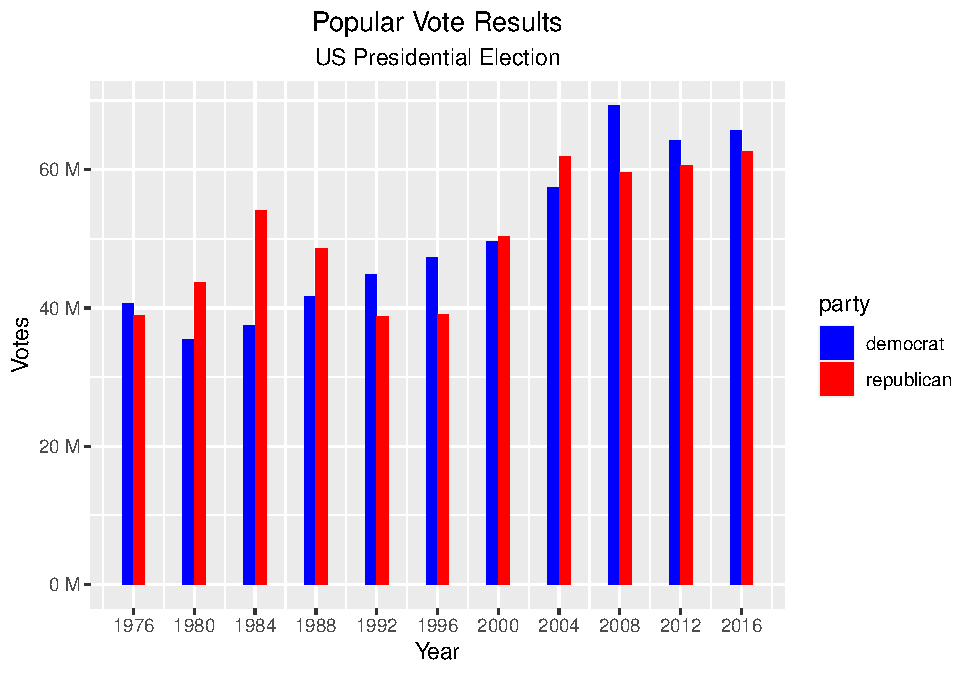
\includegraphics{election_files/figure-latex/plot1-1.pdf}

For our next trick, we will create an animation showing how the ratio of
republican democrat has shifted over time.

\begin{Shaded}
\begin{Highlighting}[]
\KeywordTok{ggplot}\NormalTok{(dvr_year) }\OperatorTok{+}
\StringTok{  }\KeywordTok{geom_bar}\NormalTok{(}\DataTypeTok{mapping =} \KeywordTok{aes}\NormalTok{(}\DataTypeTok{x =}\StringTok{""}\NormalTok{, }\DataTypeTok{y =}\NormalTok{ percentage, }\DataTypeTok{fill =}\NormalTok{ party), }\DataTypeTok{width =} \DecValTok{1}\NormalTok{, }\DataTypeTok{stat =} \StringTok{"identity"}\NormalTok{) }\OperatorTok{+}
\StringTok{  }\KeywordTok{coord_polar}\NormalTok{(}\StringTok{"y"}\NormalTok{, }\DataTypeTok{start=}\DecValTok{0}\NormalTok{) }\OperatorTok{+}
\StringTok{  }\KeywordTok{scale_fill_manual}\NormalTok{(}
    \DataTypeTok{values =} \KeywordTok{c}\NormalTok{(}\StringTok{"#0000FF"}\NormalTok{,}\StringTok{"#FF0000"}\NormalTok{)}
\NormalTok{    ) }\OperatorTok{+}
\StringTok{  }\KeywordTok{transition_states}\NormalTok{(year) }\OperatorTok{+}
\StringTok{  }\KeywordTok{labs}\NormalTok{(}
    \DataTypeTok{title =} \StringTok{"Ratio of Democrat and Republican Voters"}\NormalTok{,}
    \DataTypeTok{subtitle =} \StringTok{"Presidential Election: \{closest_state\}"}
\NormalTok{    ) }\OperatorTok{+}
\StringTok{  }\KeywordTok{theme}\NormalTok{(}
    \DataTypeTok{plot.title =} \KeywordTok{element_text}\NormalTok{(}\DataTypeTok{hjust =} \FloatTok{.5}\NormalTok{),}
    \DataTypeTok{plot.subtitle =} \KeywordTok{element_text}\NormalTok{(}\DataTypeTok{hjust =} \FloatTok{.5}\NormalTok{)}
\NormalTok{  )}
\end{Highlighting}
\end{Shaded}

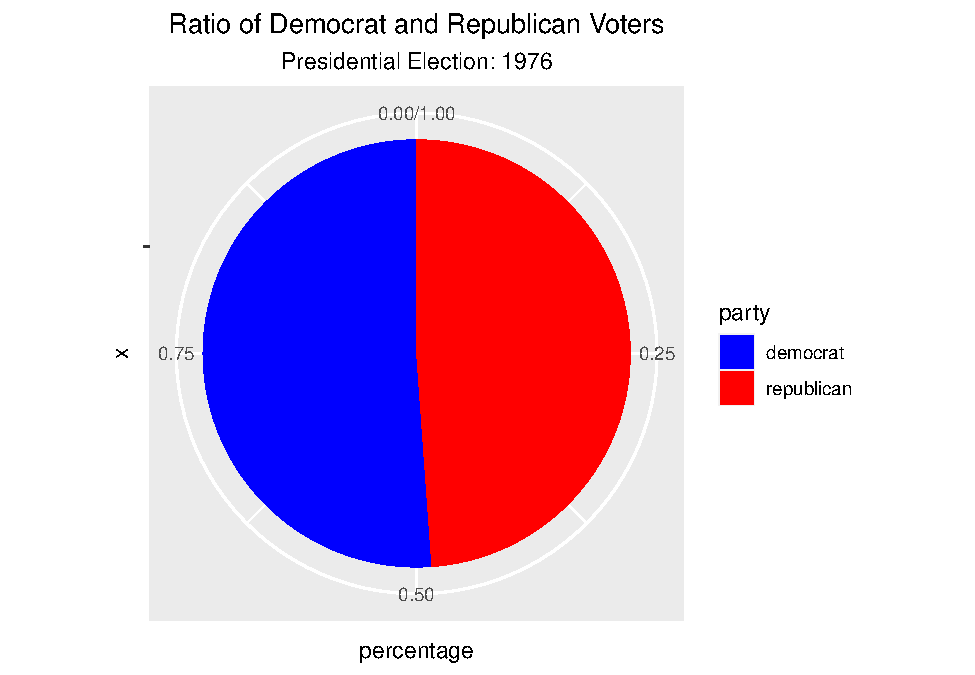
\includegraphics{election_files/figure-latex/anim-1.pdf}
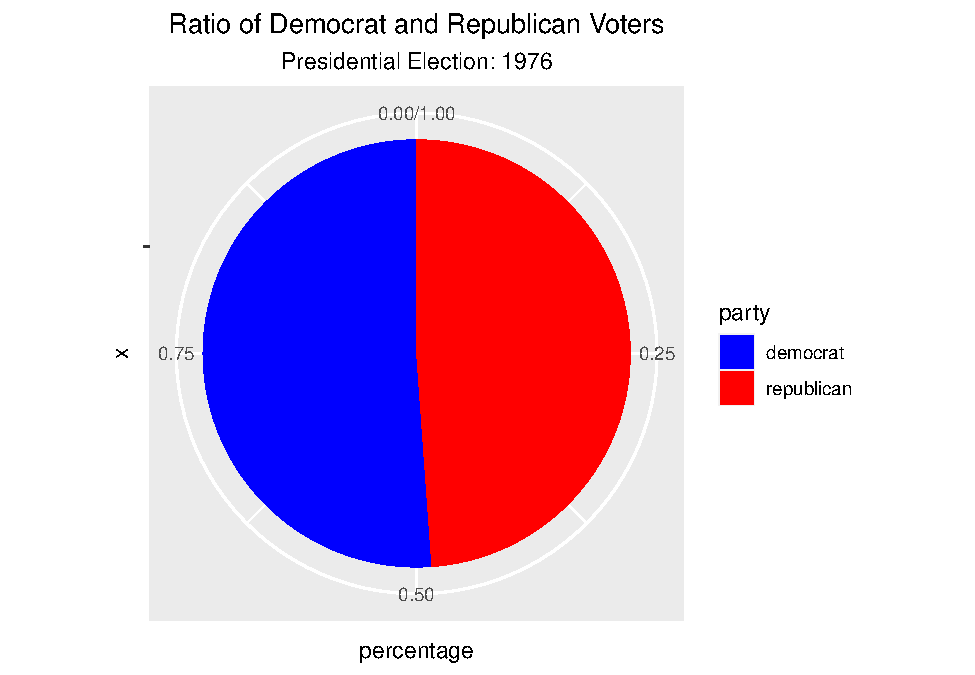
\includegraphics{election_files/figure-latex/anim-2.pdf}
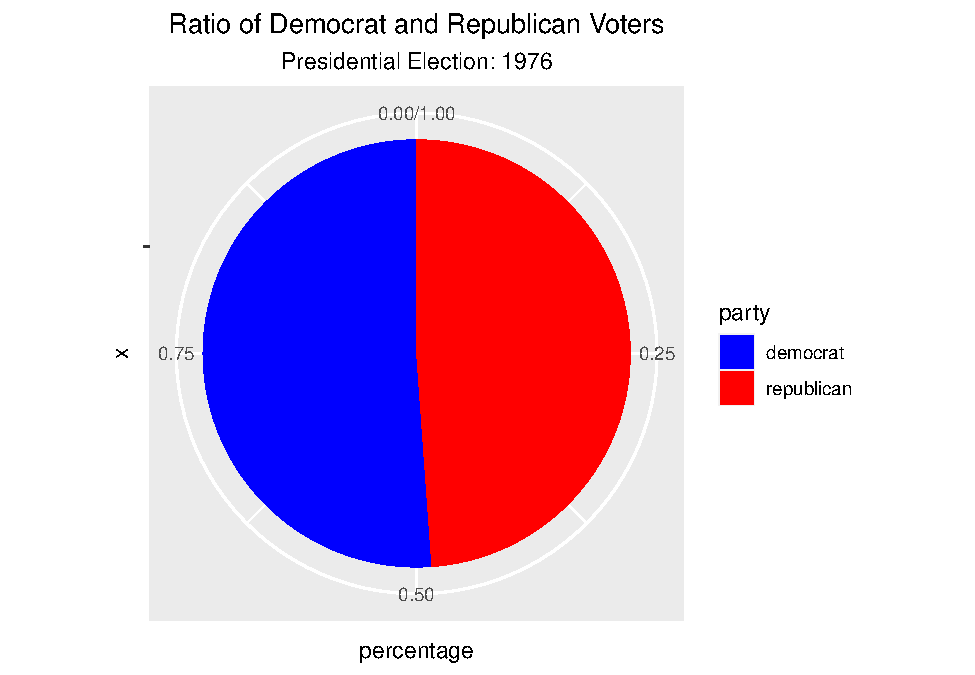
\includegraphics{election_files/figure-latex/anim-3.pdf}
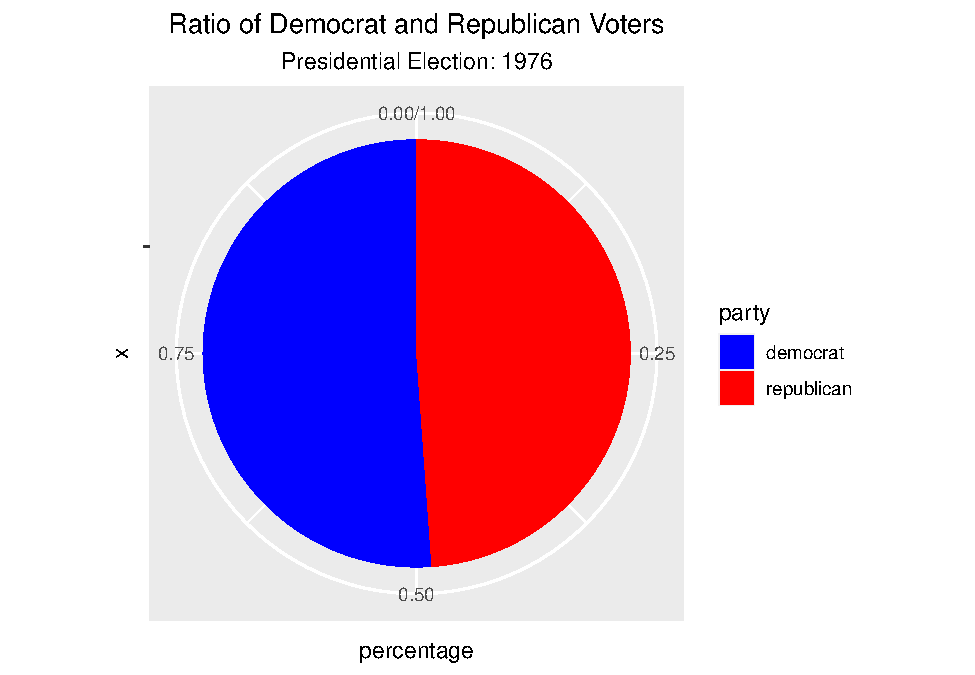
\includegraphics{election_files/figure-latex/anim-4.pdf}
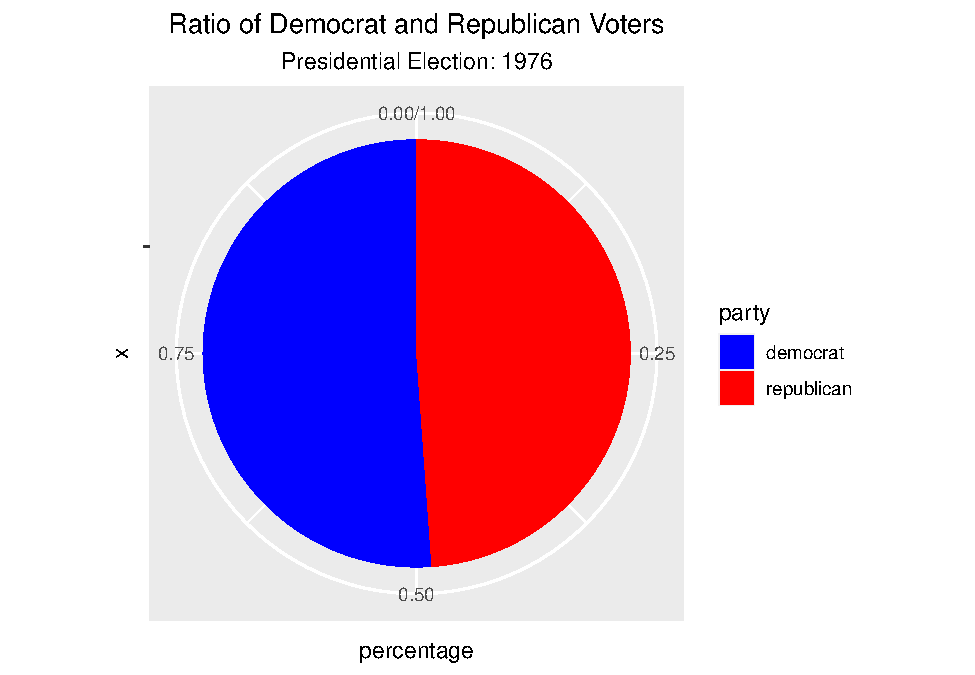
\includegraphics{election_files/figure-latex/anim-5.pdf}
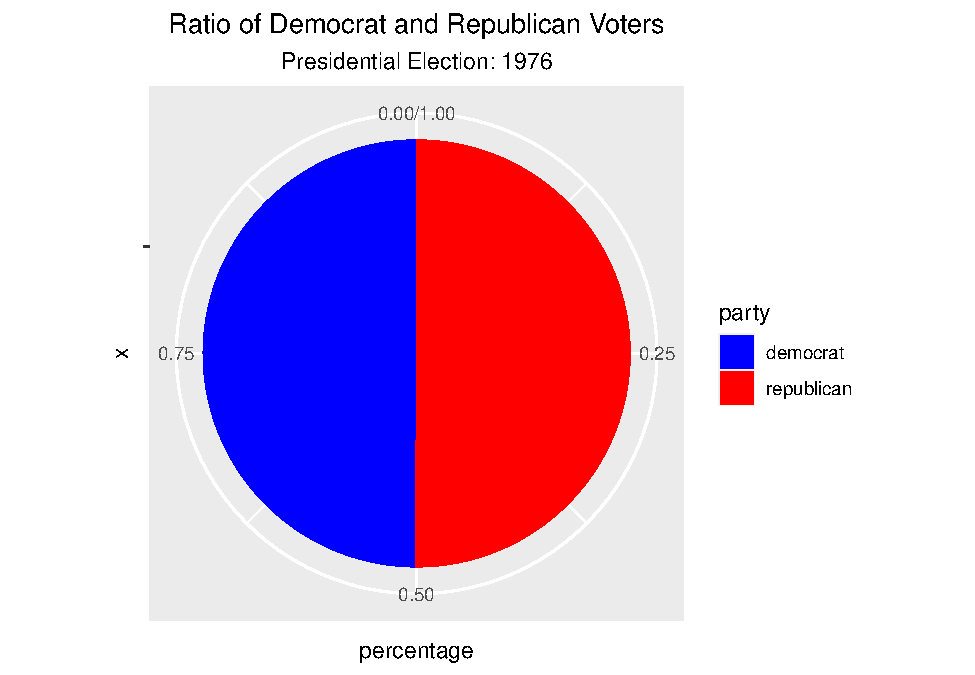
\includegraphics{election_files/figure-latex/anim-6.pdf}
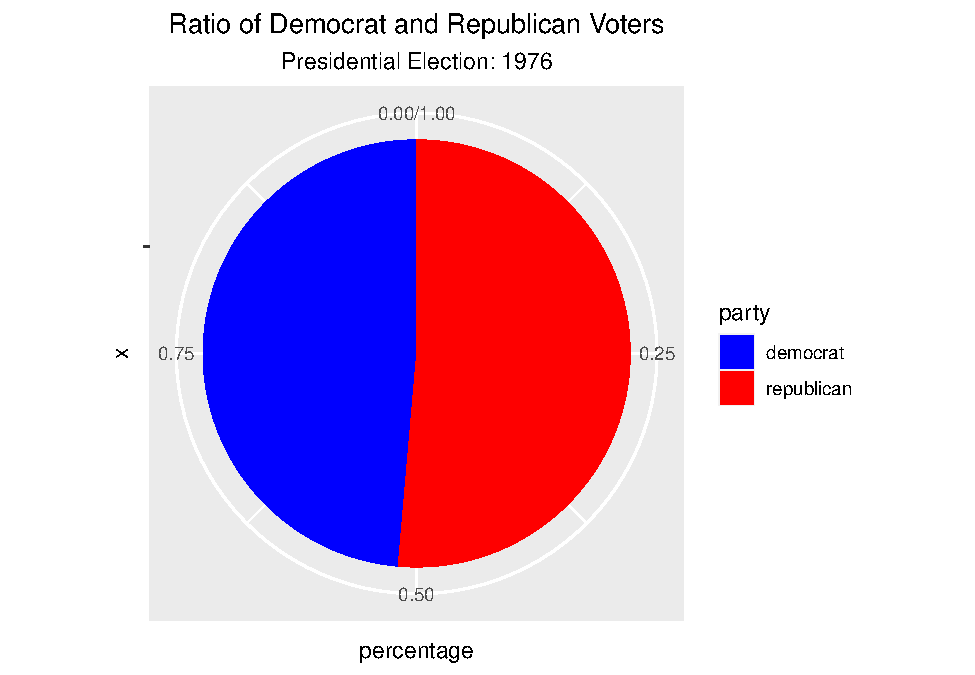
\includegraphics{election_files/figure-latex/anim-7.pdf}
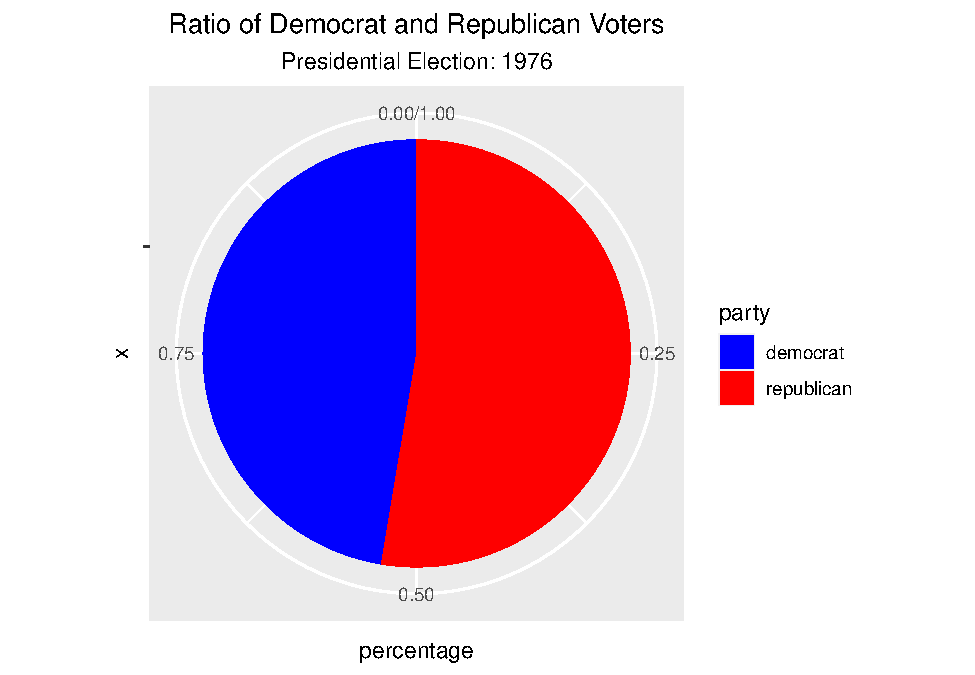
\includegraphics{election_files/figure-latex/anim-8.pdf}
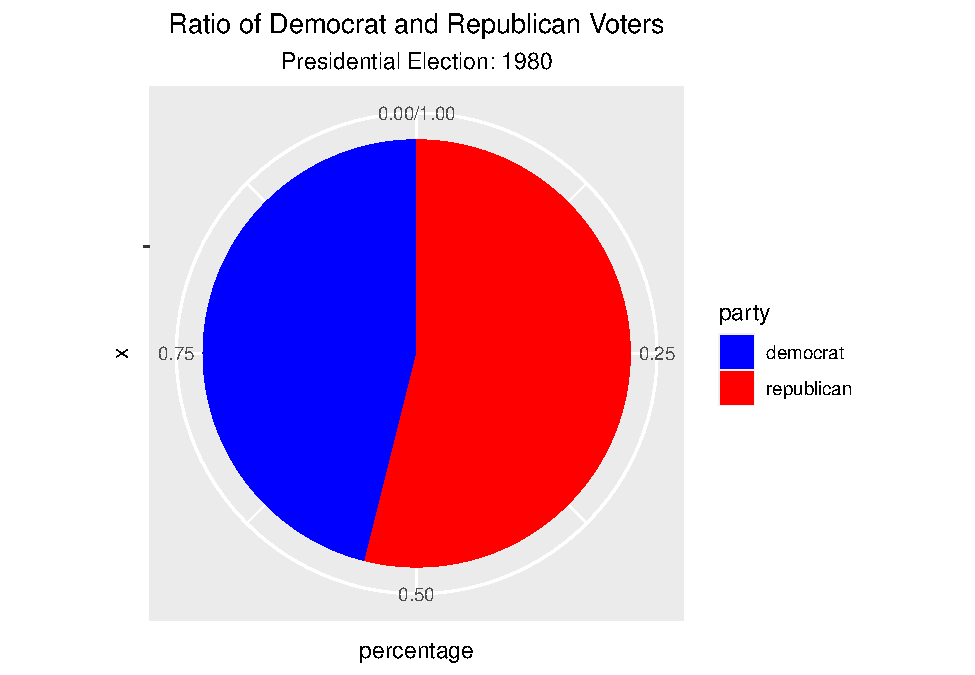
\includegraphics{election_files/figure-latex/anim-9.pdf}
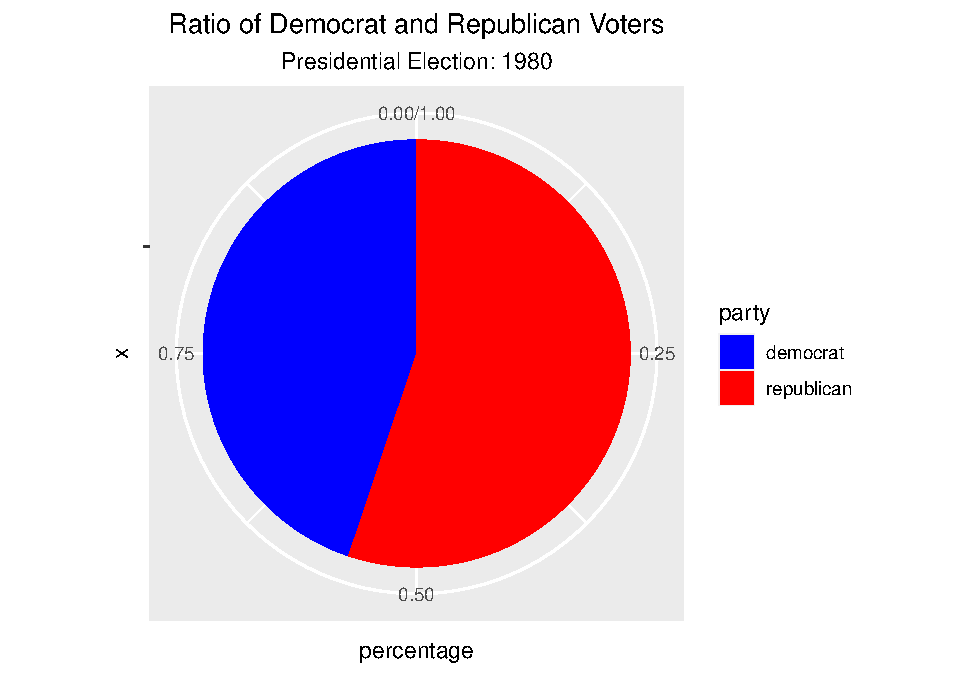
\includegraphics{election_files/figure-latex/anim-10.pdf}
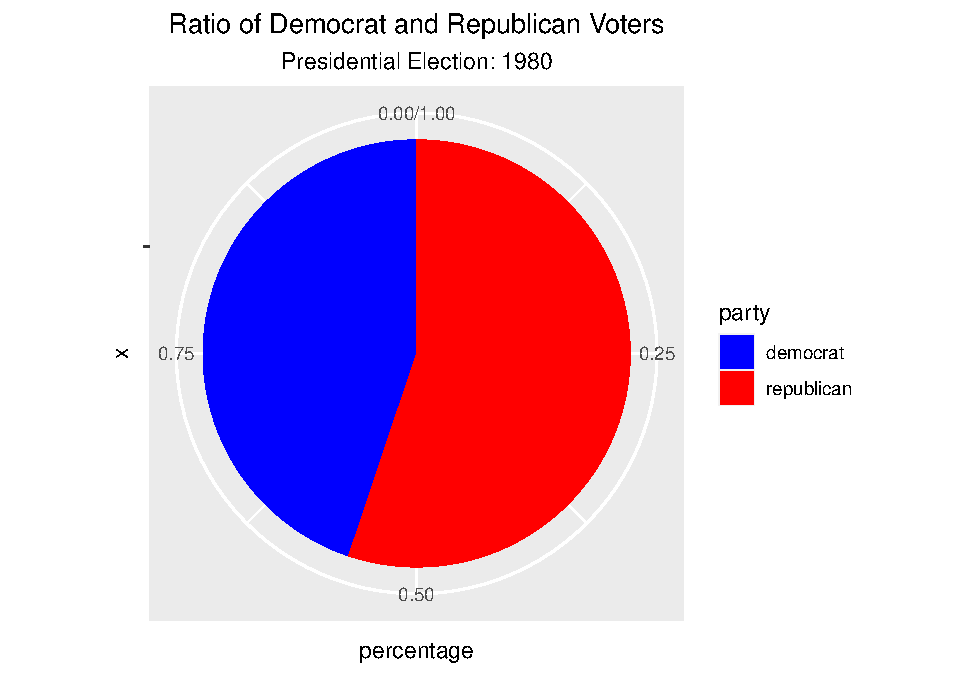
\includegraphics{election_files/figure-latex/anim-11.pdf}
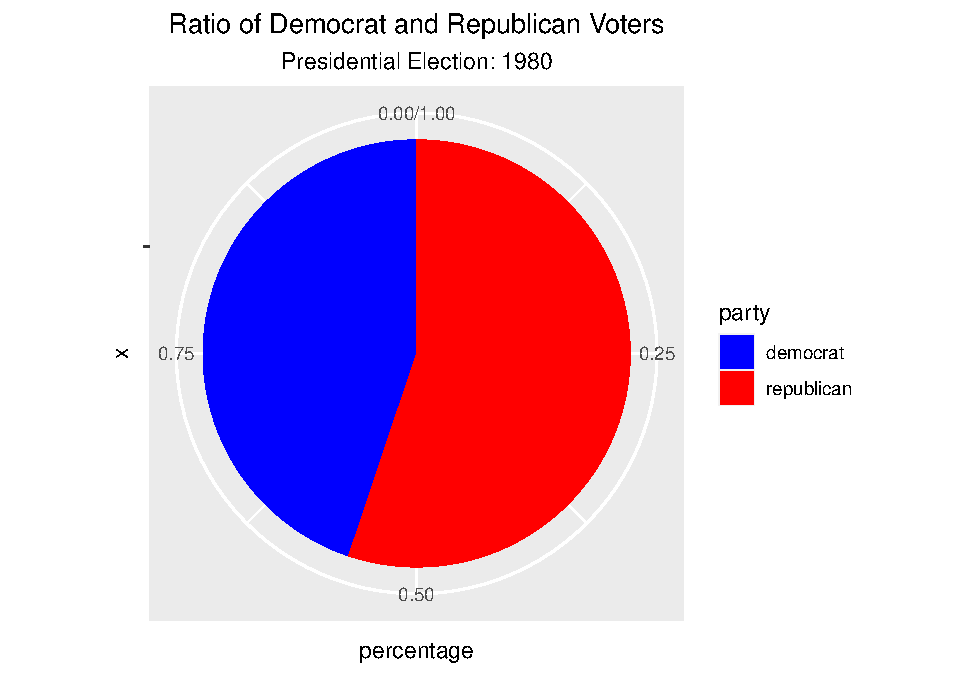
\includegraphics{election_files/figure-latex/anim-12.pdf}
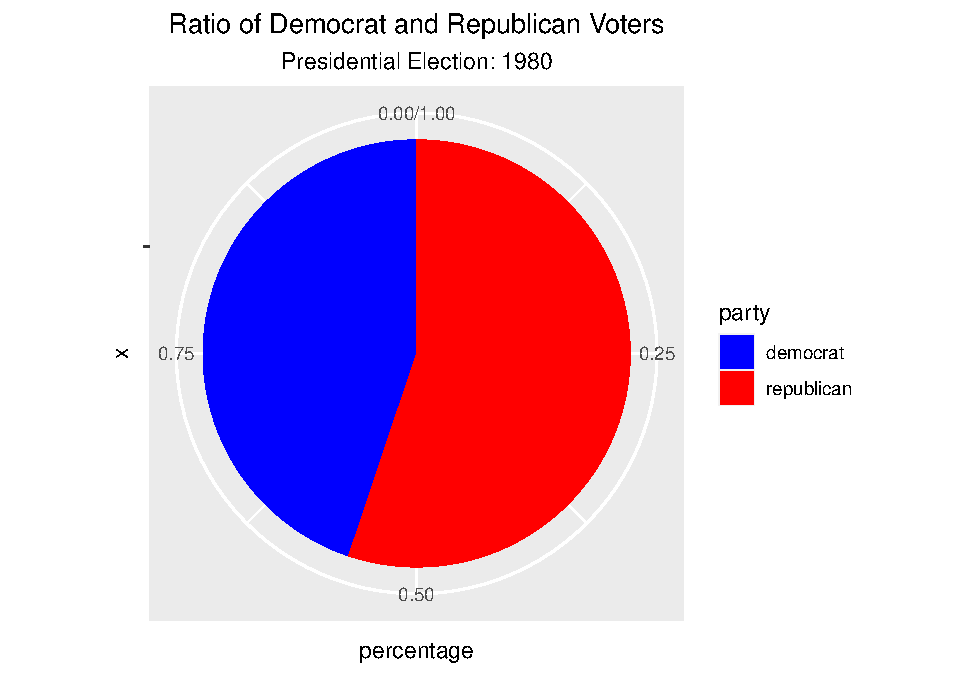
\includegraphics{election_files/figure-latex/anim-13.pdf}
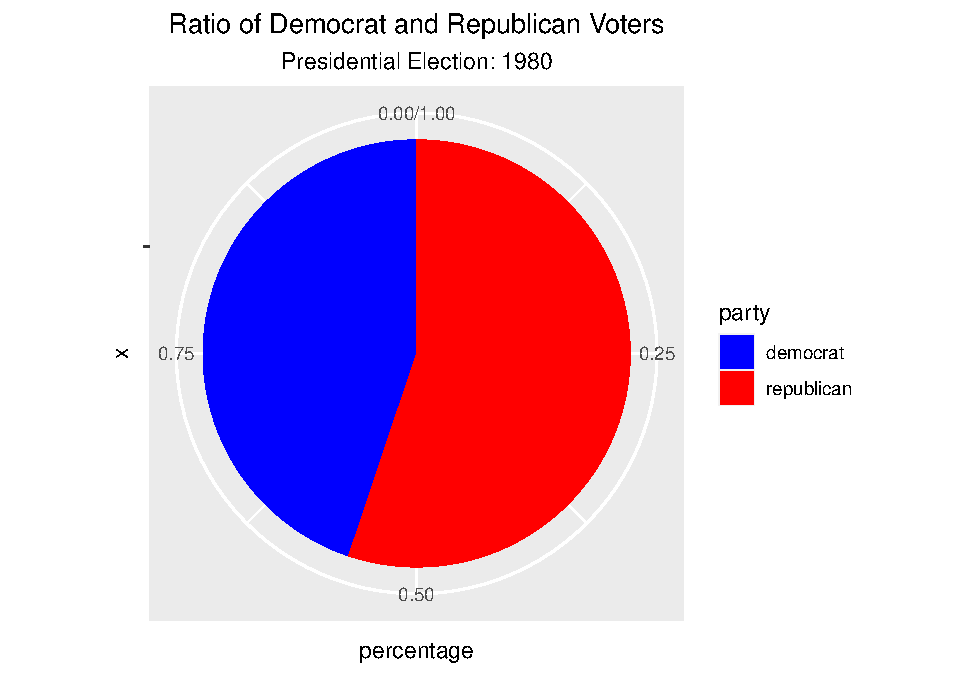
\includegraphics{election_files/figure-latex/anim-14.pdf}
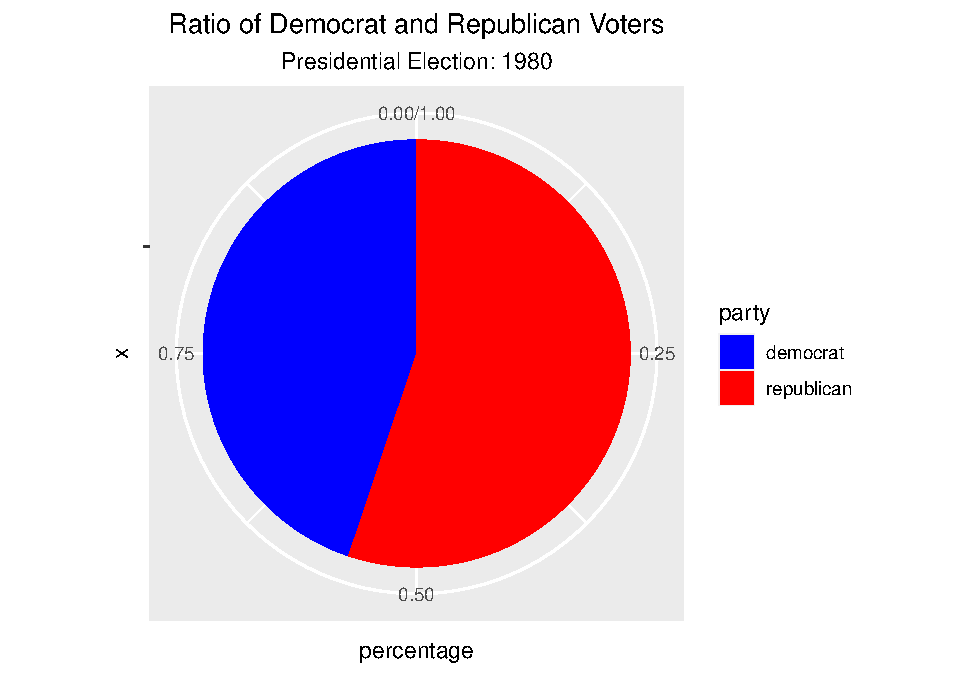
\includegraphics{election_files/figure-latex/anim-15.pdf}
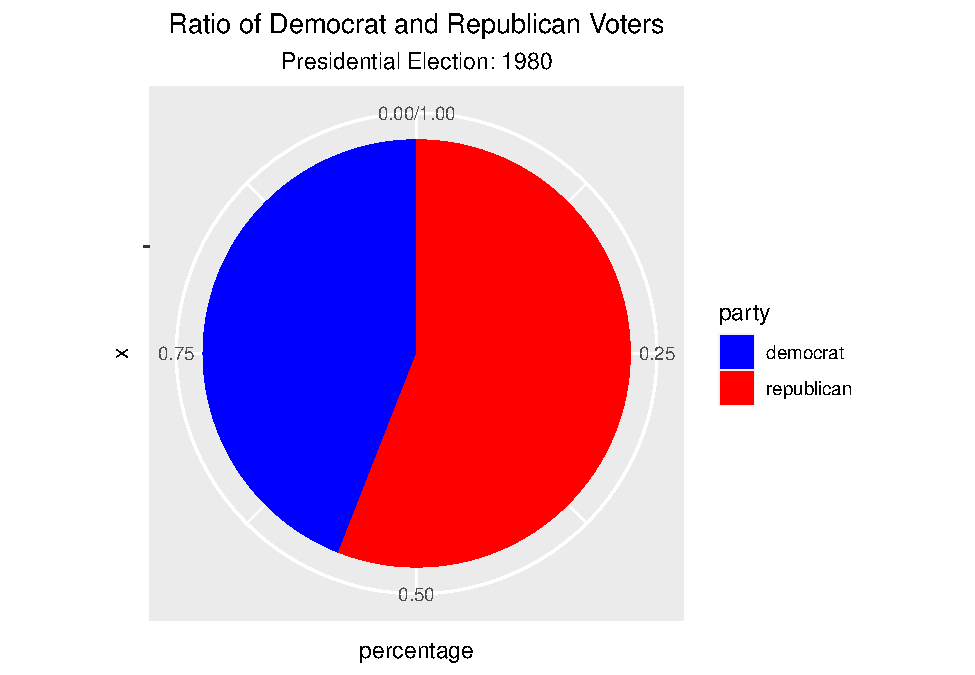
\includegraphics{election_files/figure-latex/anim-16.pdf}
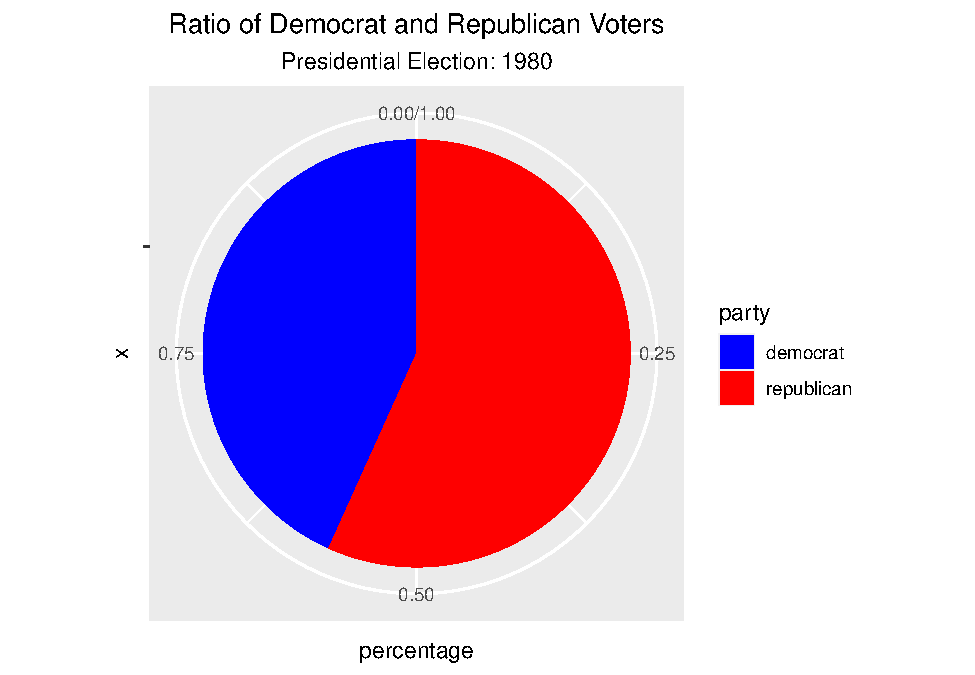
\includegraphics{election_files/figure-latex/anim-17.pdf}
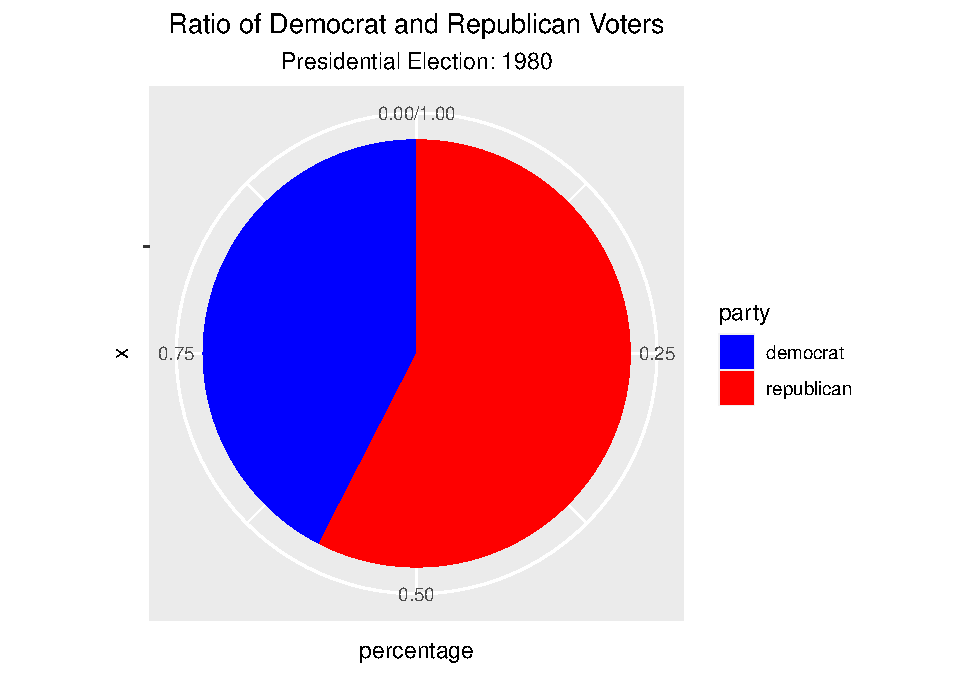
\includegraphics{election_files/figure-latex/anim-18.pdf}
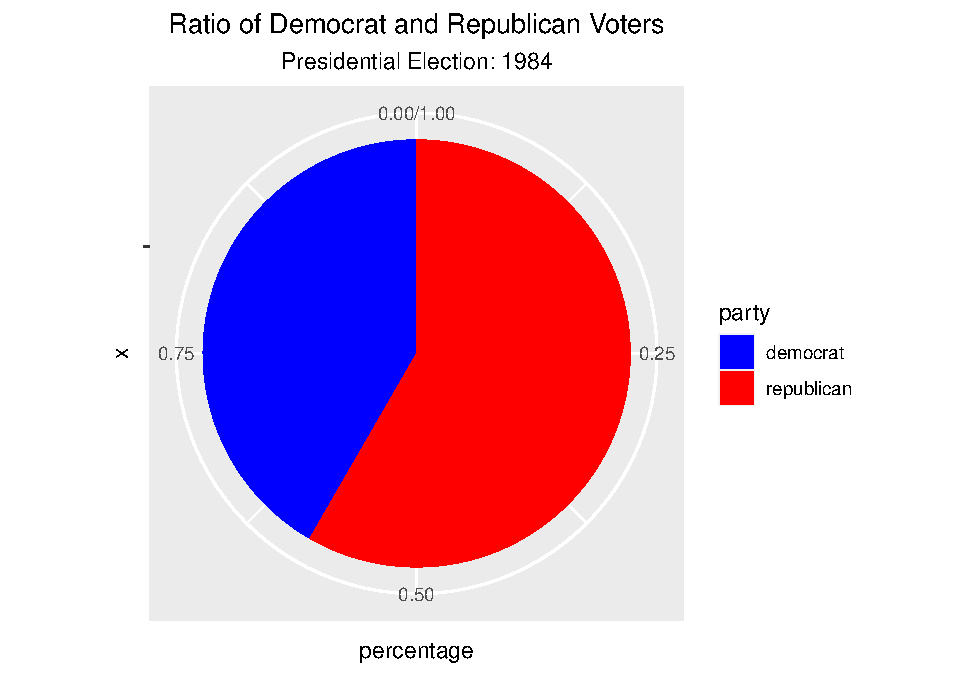
\includegraphics{election_files/figure-latex/anim-19.pdf}
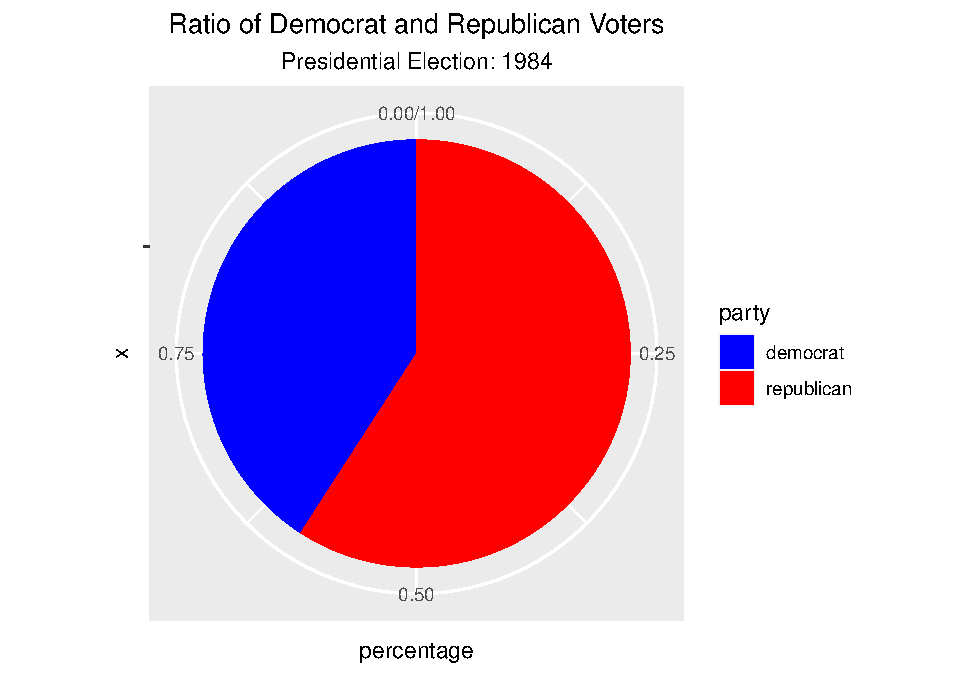
\includegraphics{election_files/figure-latex/anim-20.pdf}
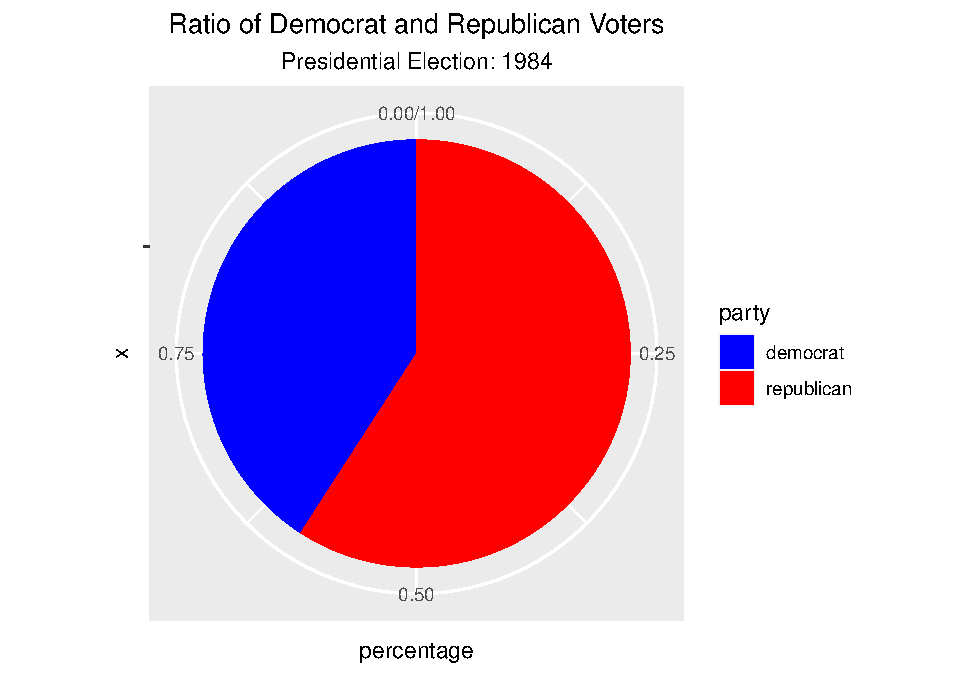
\includegraphics{election_files/figure-latex/anim-21.pdf}
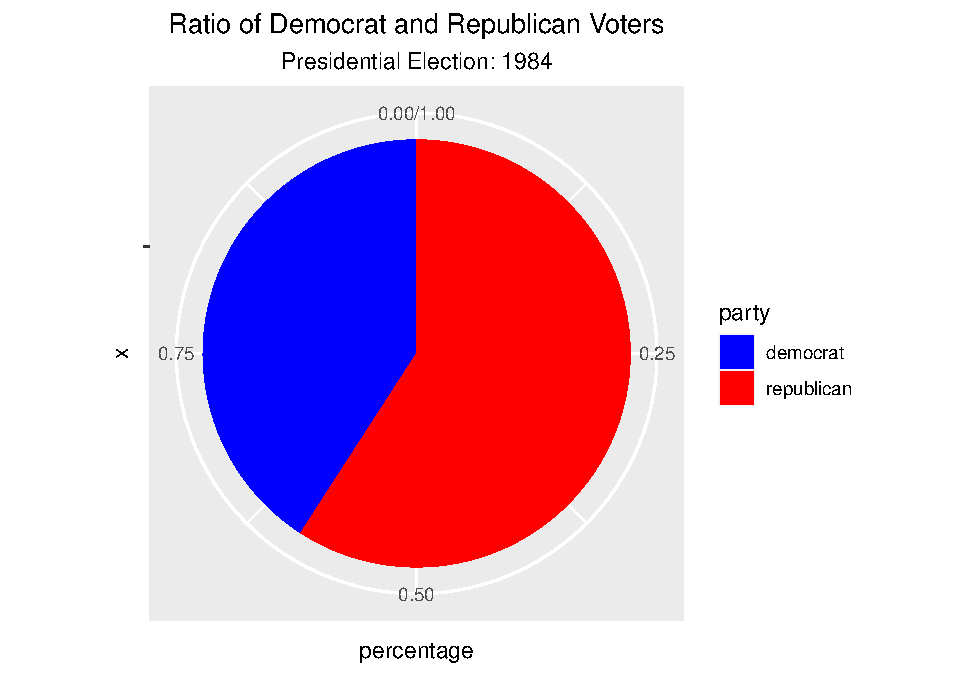
\includegraphics{election_files/figure-latex/anim-22.pdf}
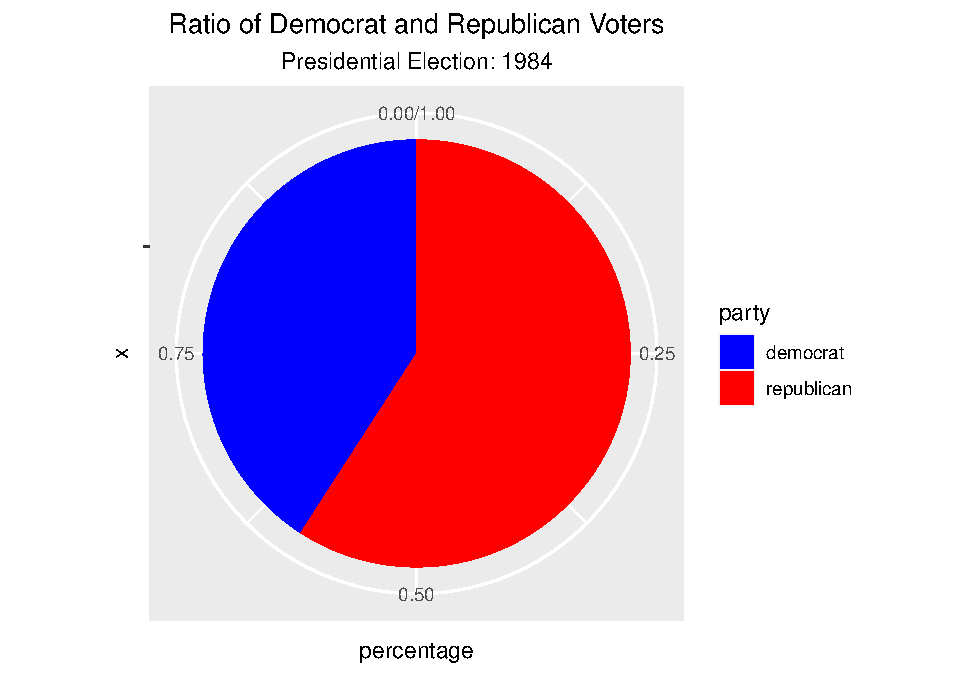
\includegraphics{election_files/figure-latex/anim-23.pdf}
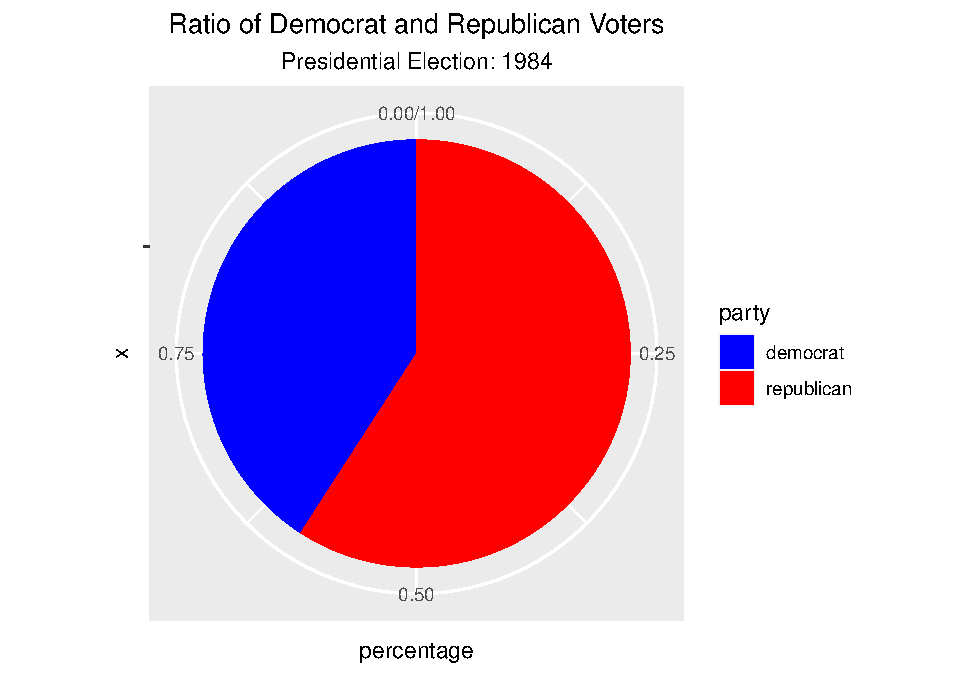
\includegraphics{election_files/figure-latex/anim-24.pdf}
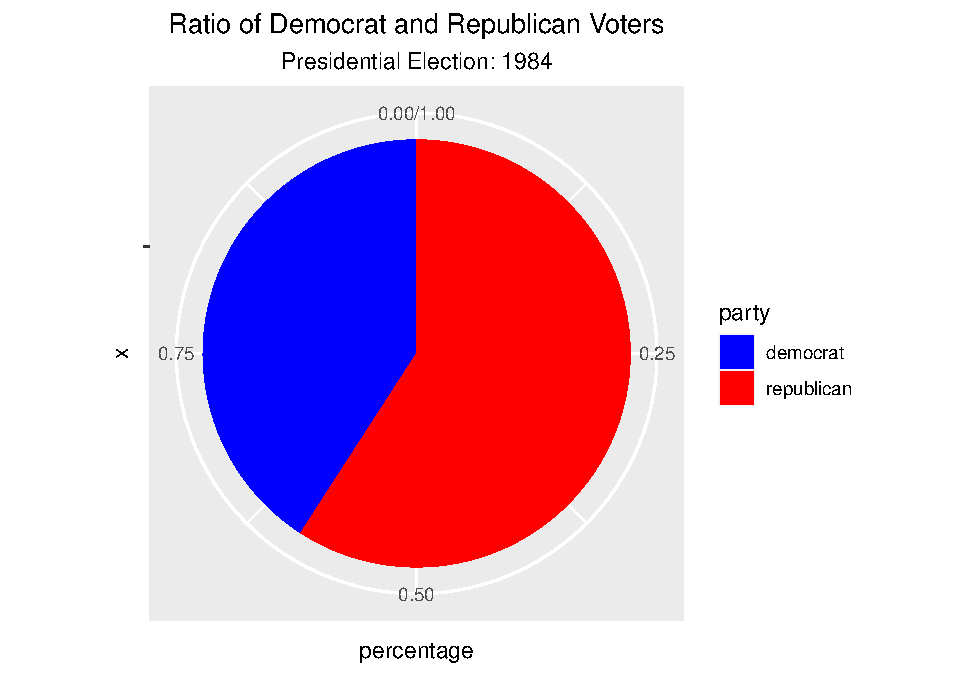
\includegraphics{election_files/figure-latex/anim-25.pdf}
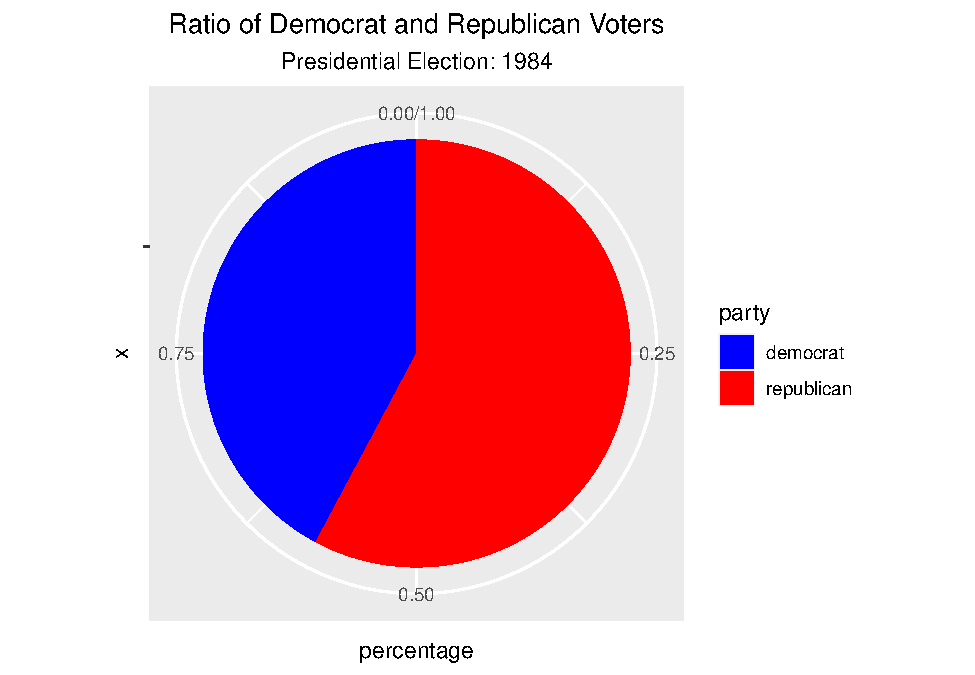
\includegraphics{election_files/figure-latex/anim-26.pdf}
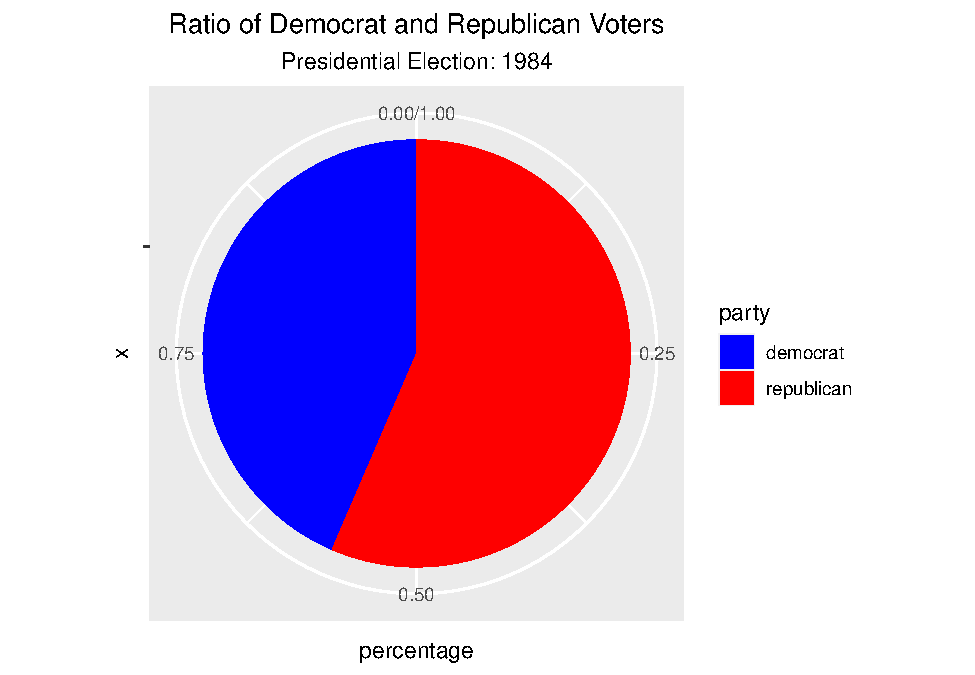
\includegraphics{election_files/figure-latex/anim-27.pdf}
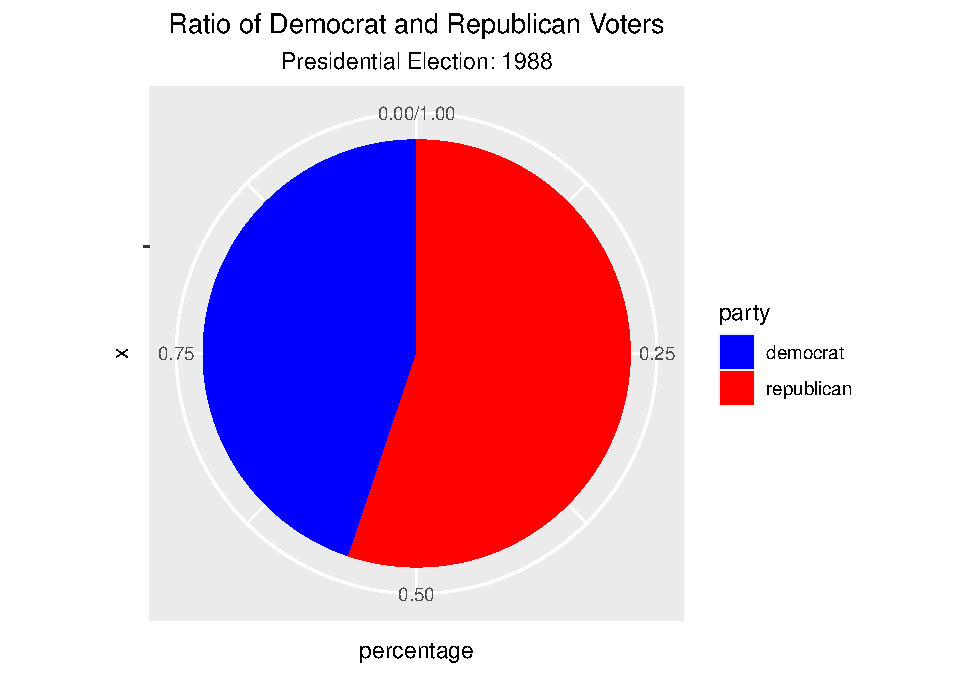
\includegraphics{election_files/figure-latex/anim-28.pdf}
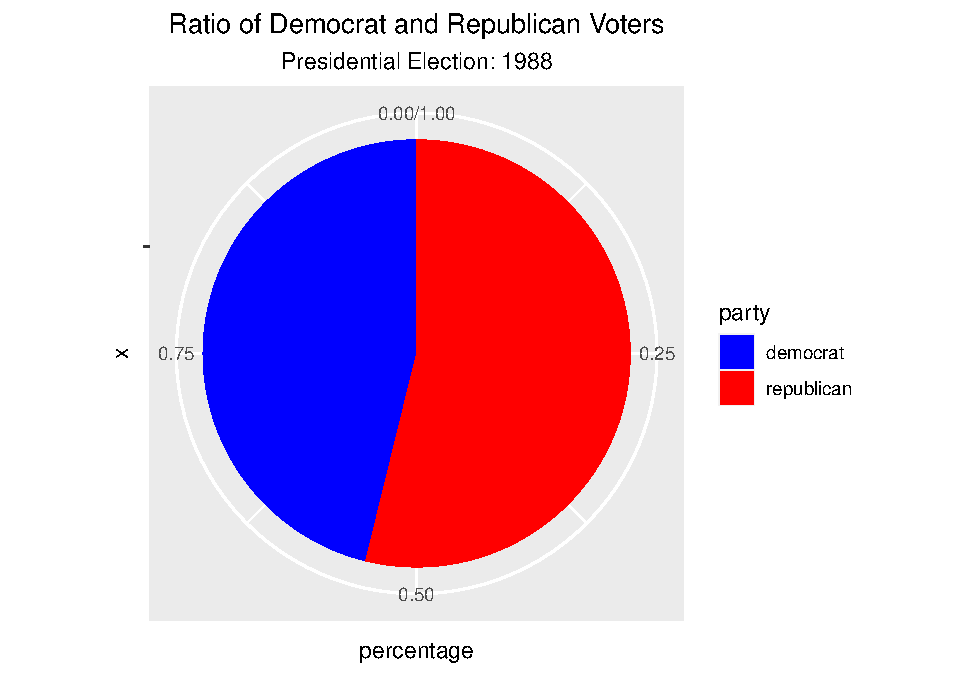
\includegraphics{election_files/figure-latex/anim-29.pdf}
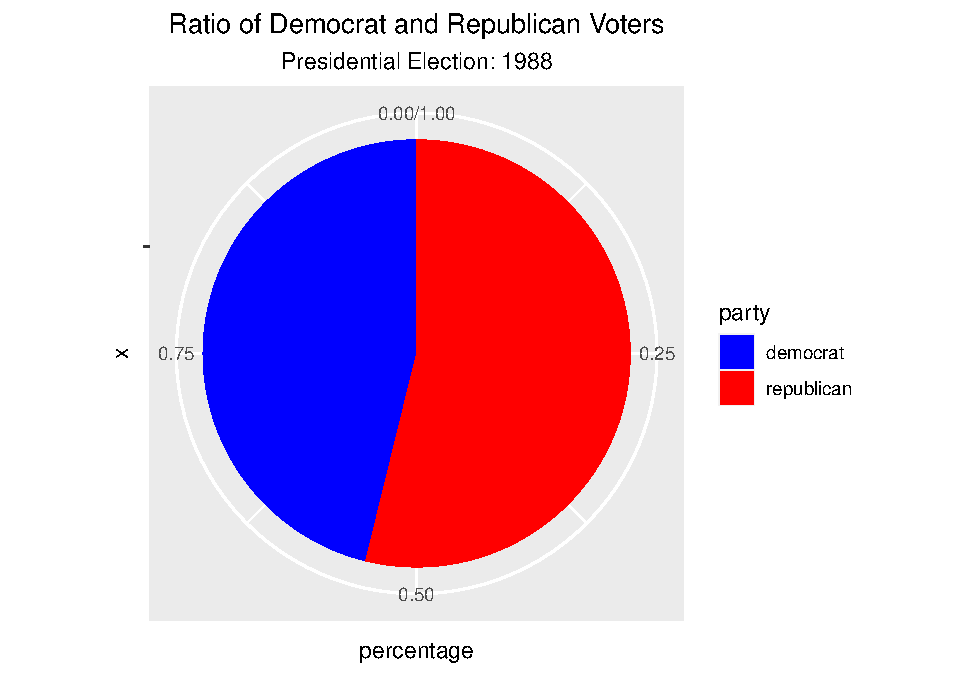
\includegraphics{election_files/figure-latex/anim-30.pdf}
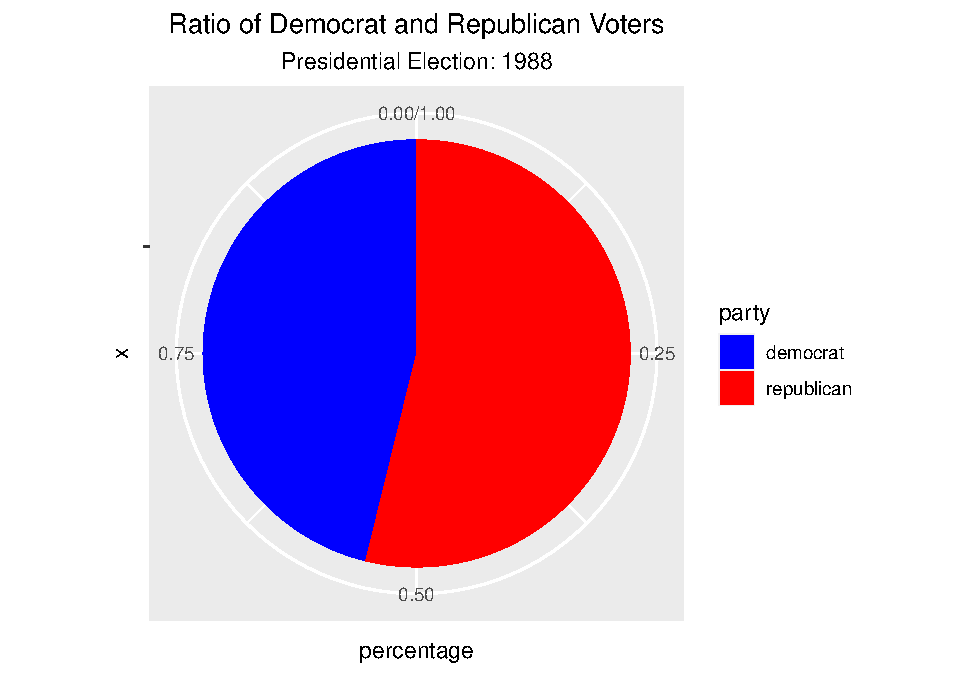
\includegraphics{election_files/figure-latex/anim-31.pdf}
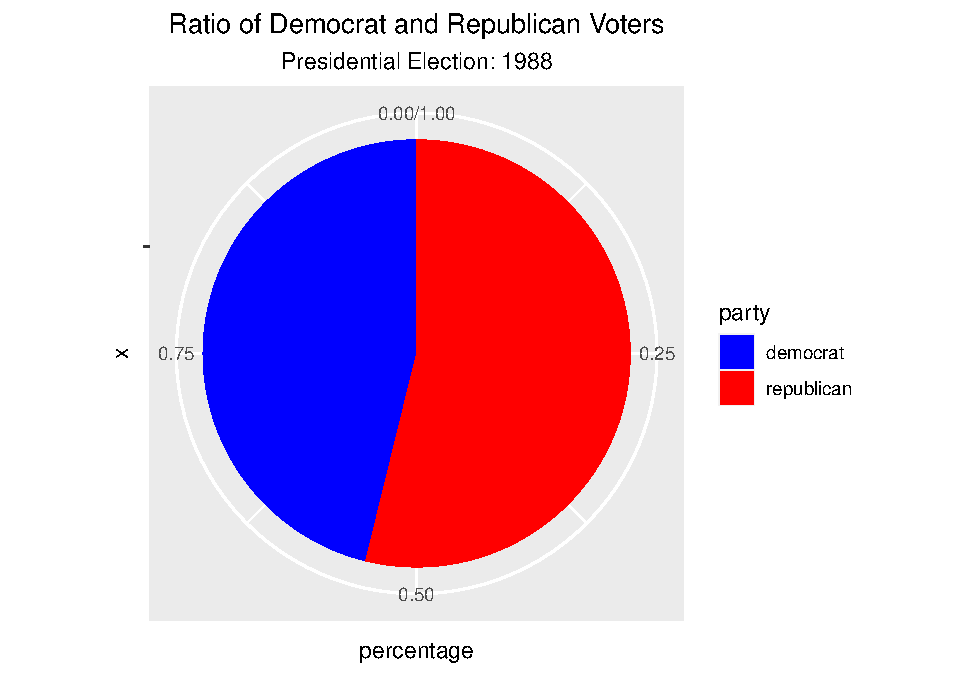
\includegraphics{election_files/figure-latex/anim-32.pdf}
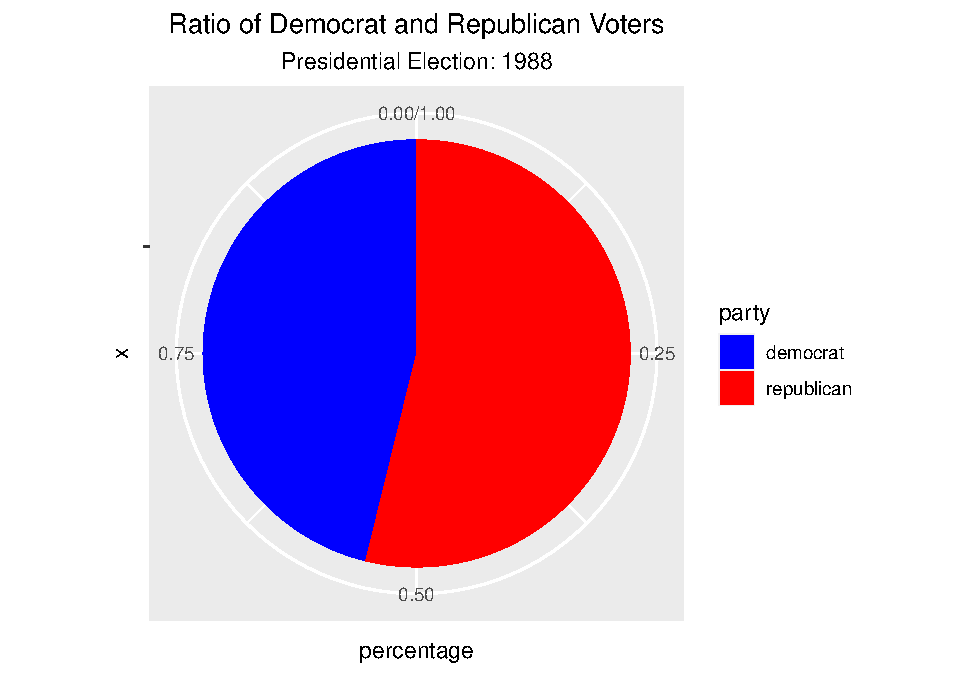
\includegraphics{election_files/figure-latex/anim-33.pdf}
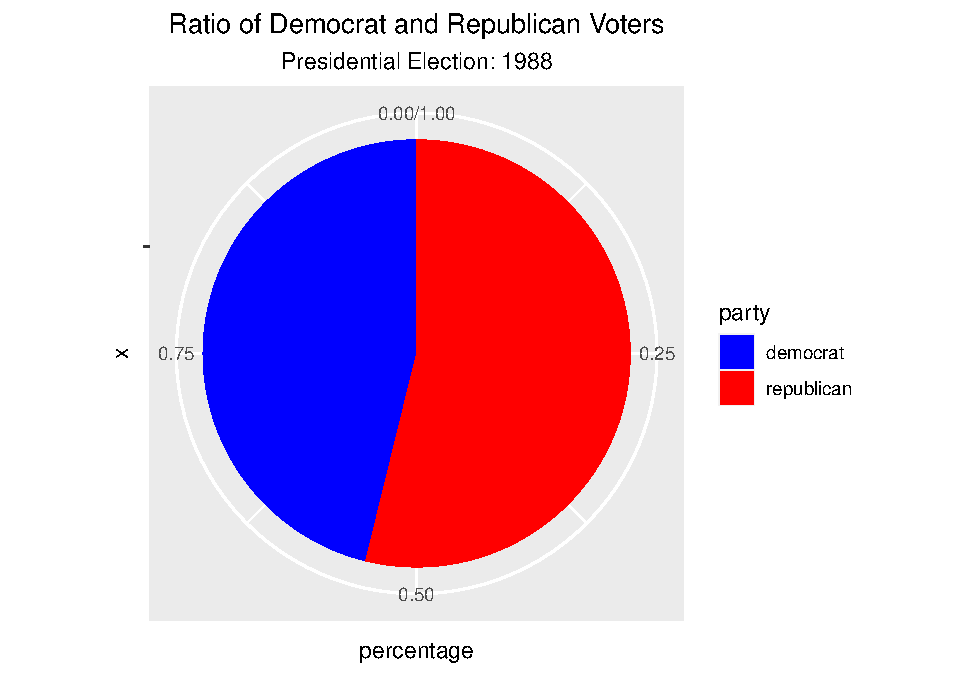
\includegraphics{election_files/figure-latex/anim-34.pdf}
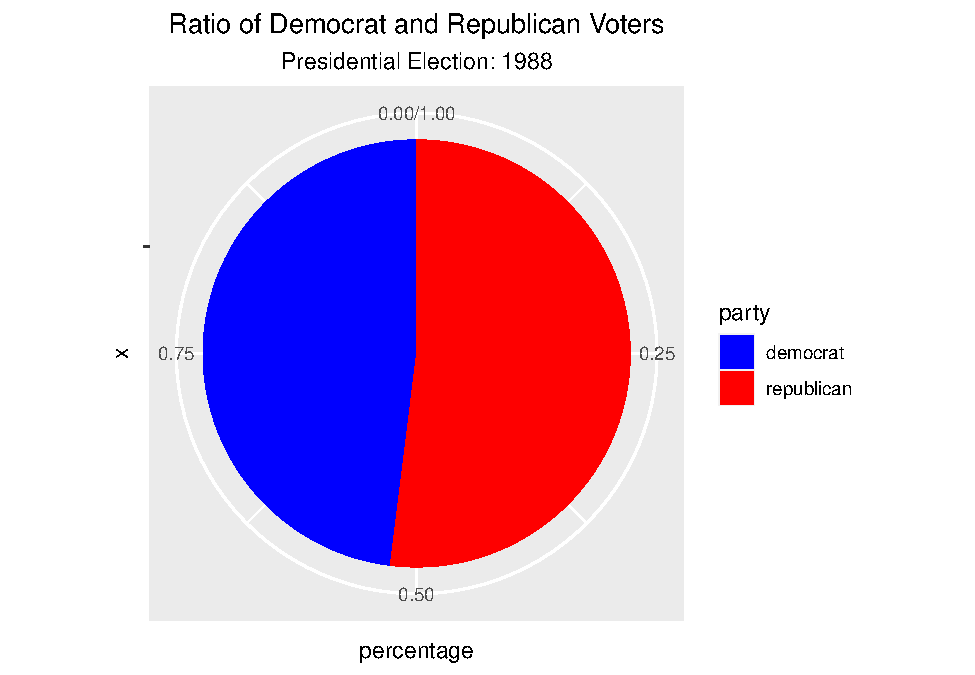
\includegraphics{election_files/figure-latex/anim-35.pdf}
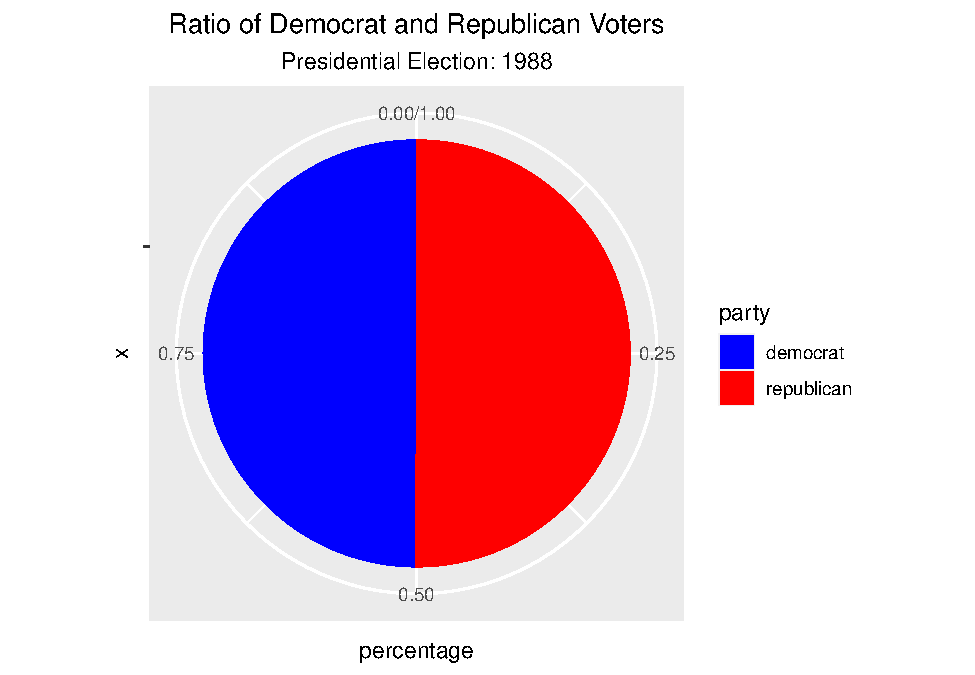
\includegraphics{election_files/figure-latex/anim-36.pdf}
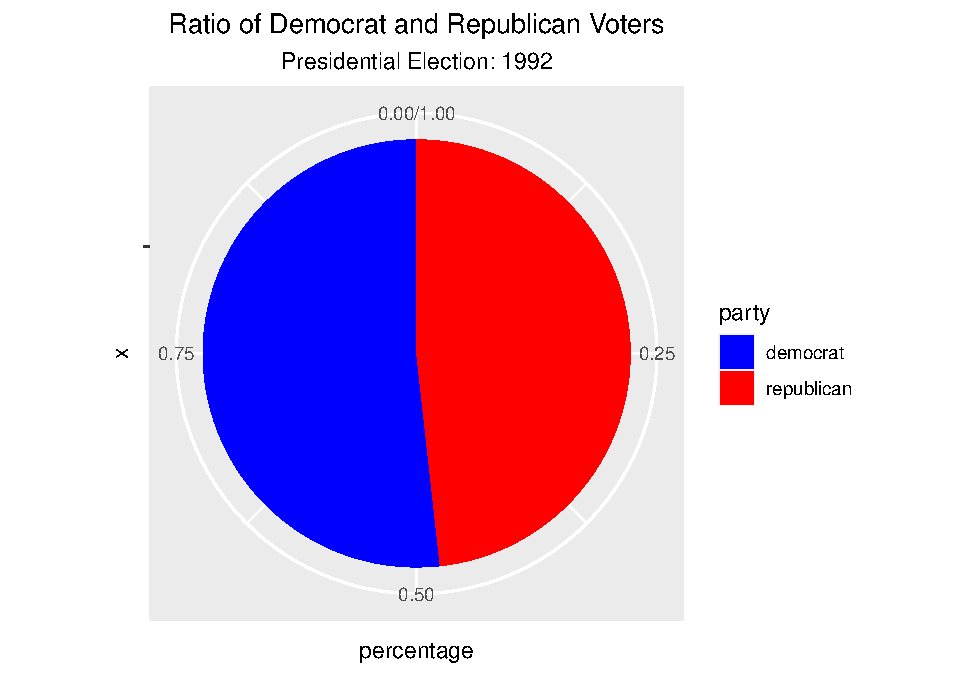
\includegraphics{election_files/figure-latex/anim-37.pdf}
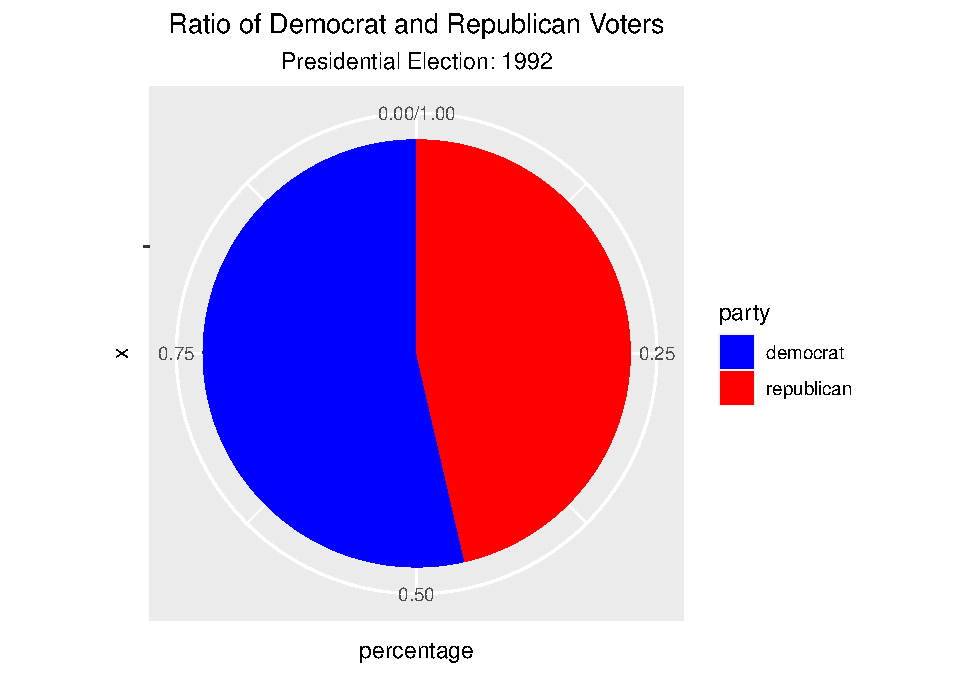
\includegraphics{election_files/figure-latex/anim-38.pdf}
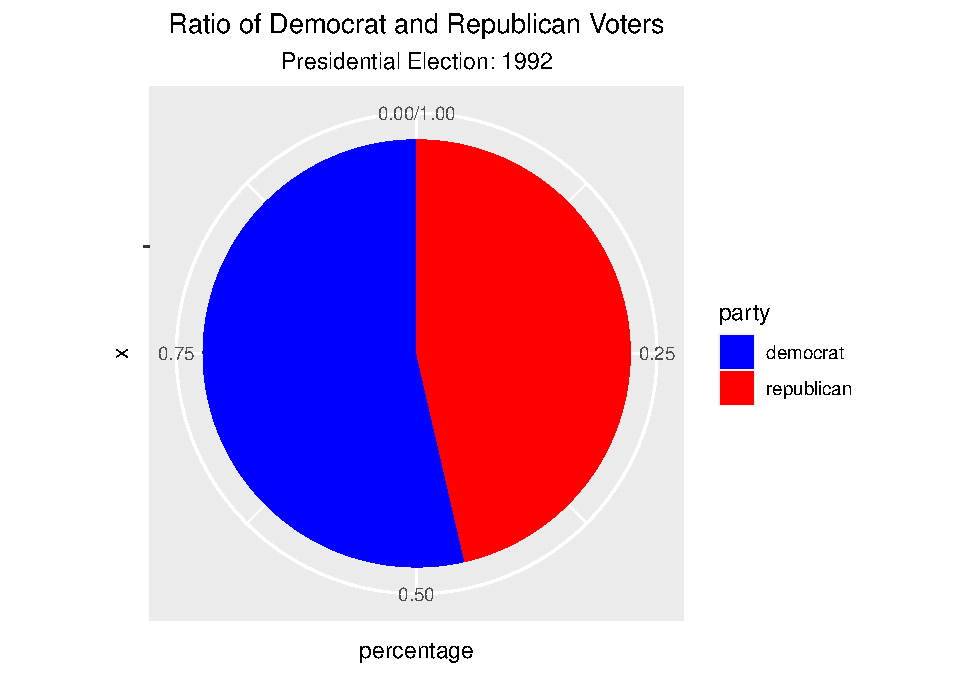
\includegraphics{election_files/figure-latex/anim-39.pdf}
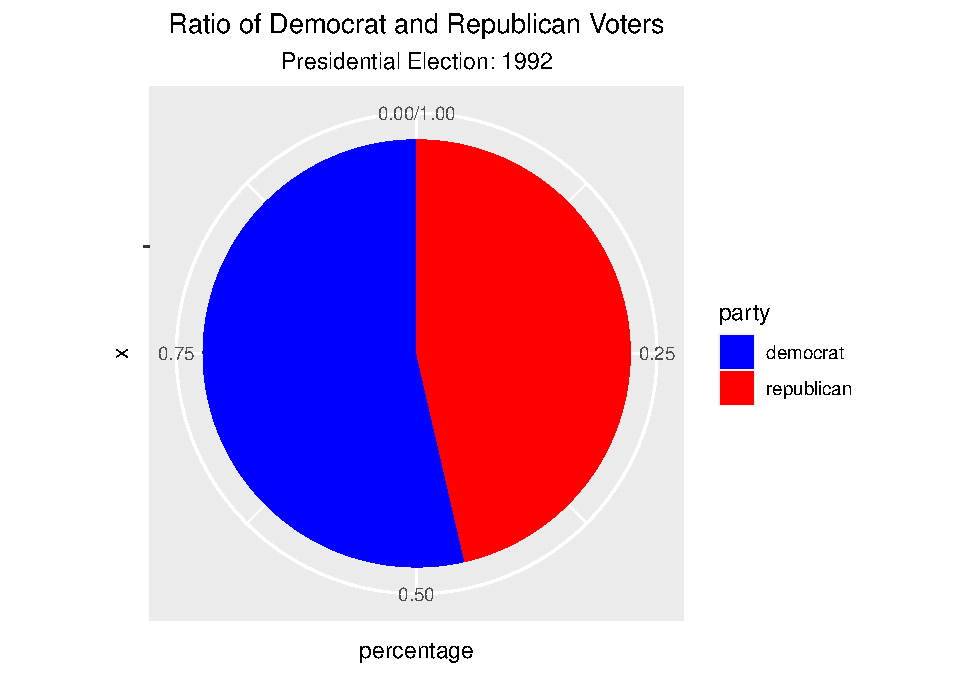
\includegraphics{election_files/figure-latex/anim-40.pdf}
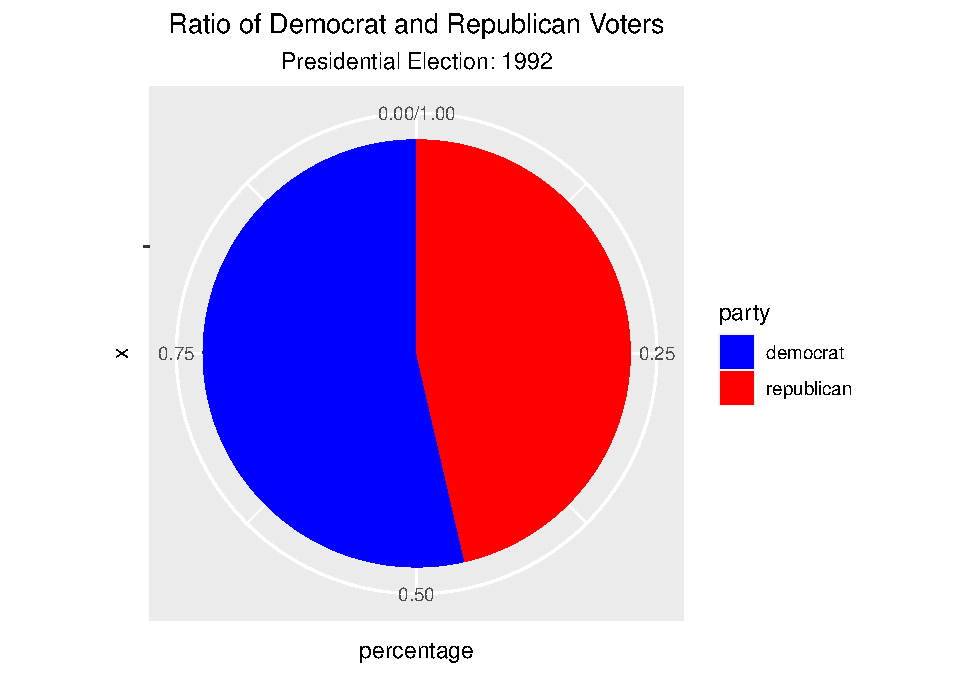
\includegraphics{election_files/figure-latex/anim-41.pdf}
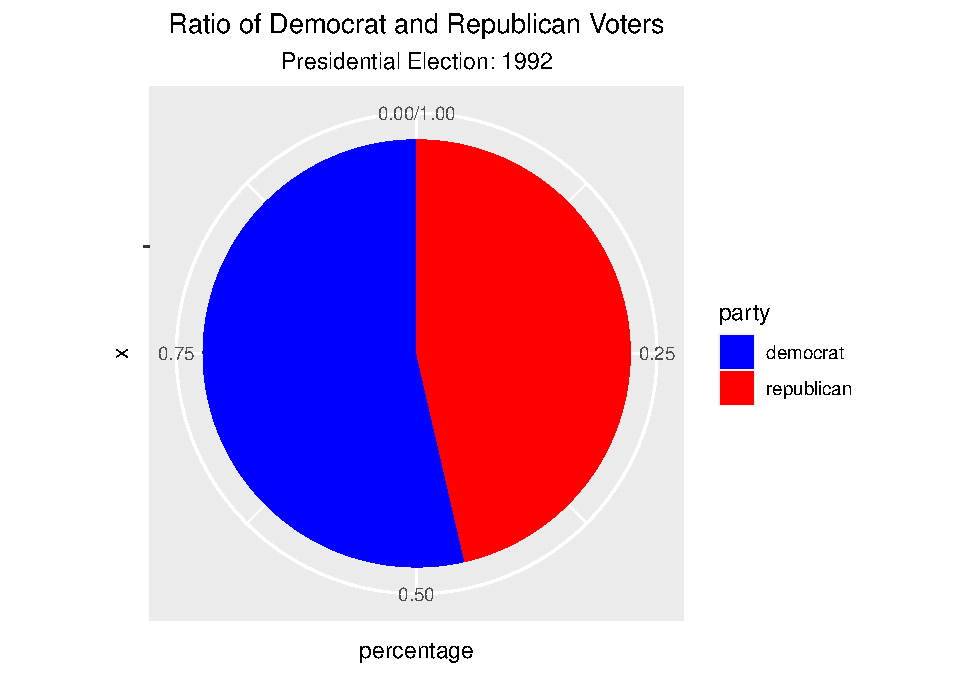
\includegraphics{election_files/figure-latex/anim-42.pdf}
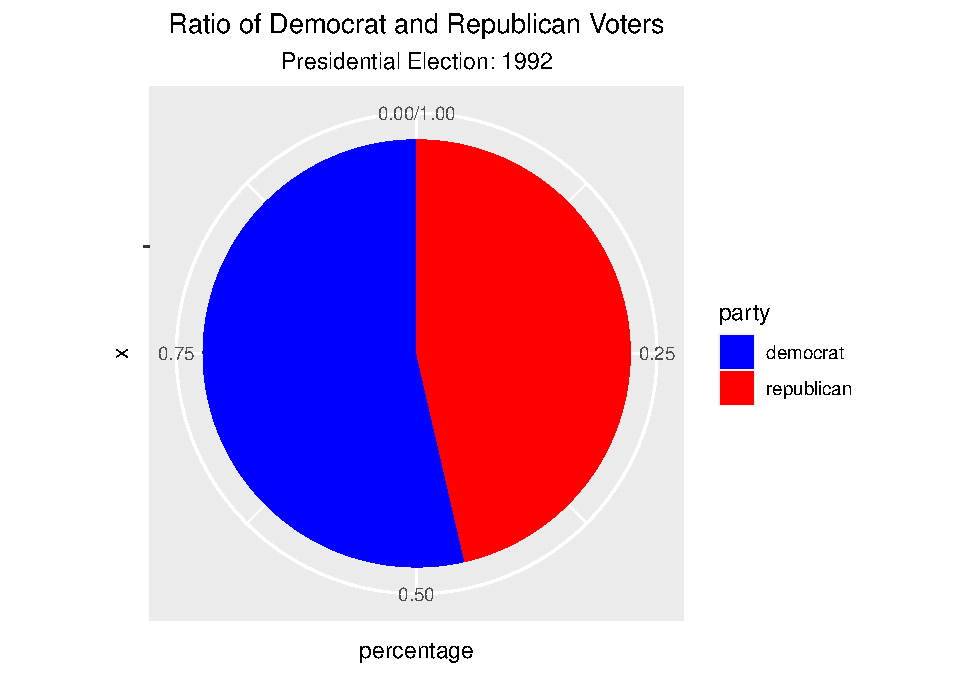
\includegraphics{election_files/figure-latex/anim-43.pdf}
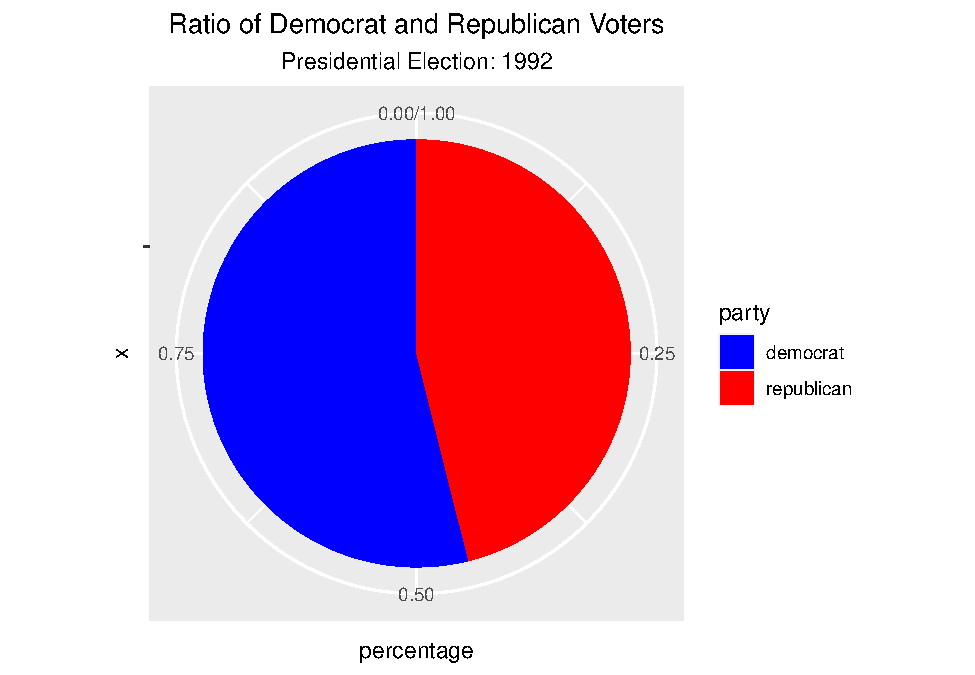
\includegraphics{election_files/figure-latex/anim-44.pdf}
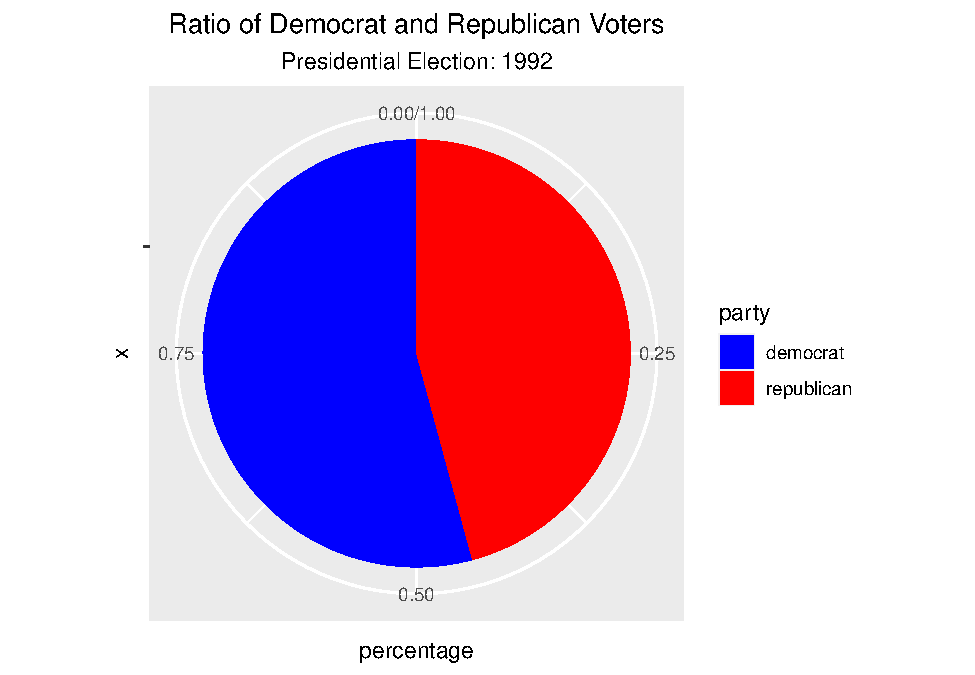
\includegraphics{election_files/figure-latex/anim-45.pdf}
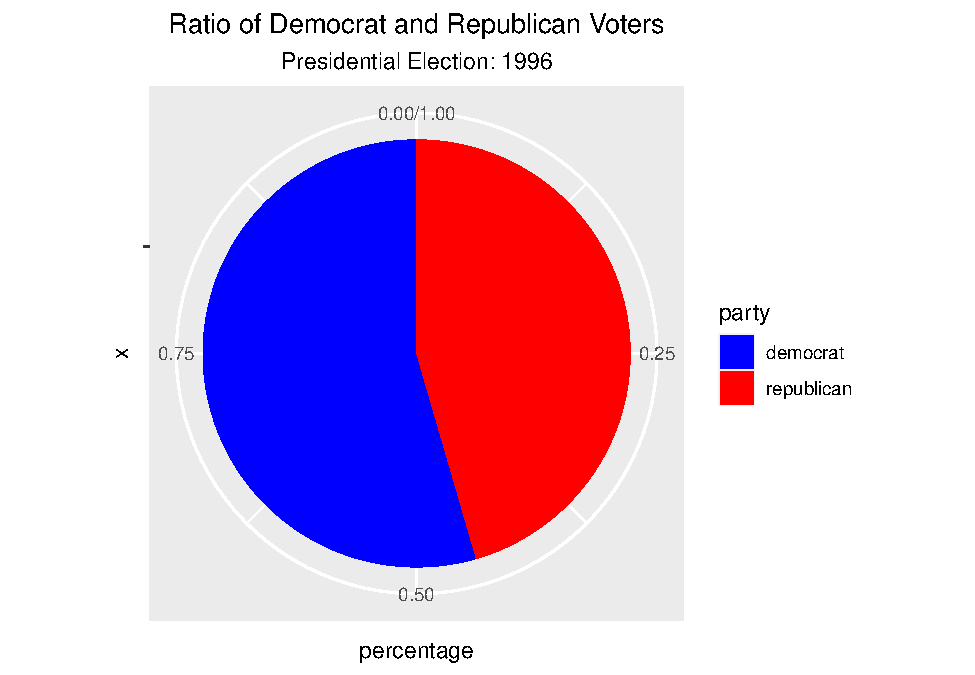
\includegraphics{election_files/figure-latex/anim-46.pdf}
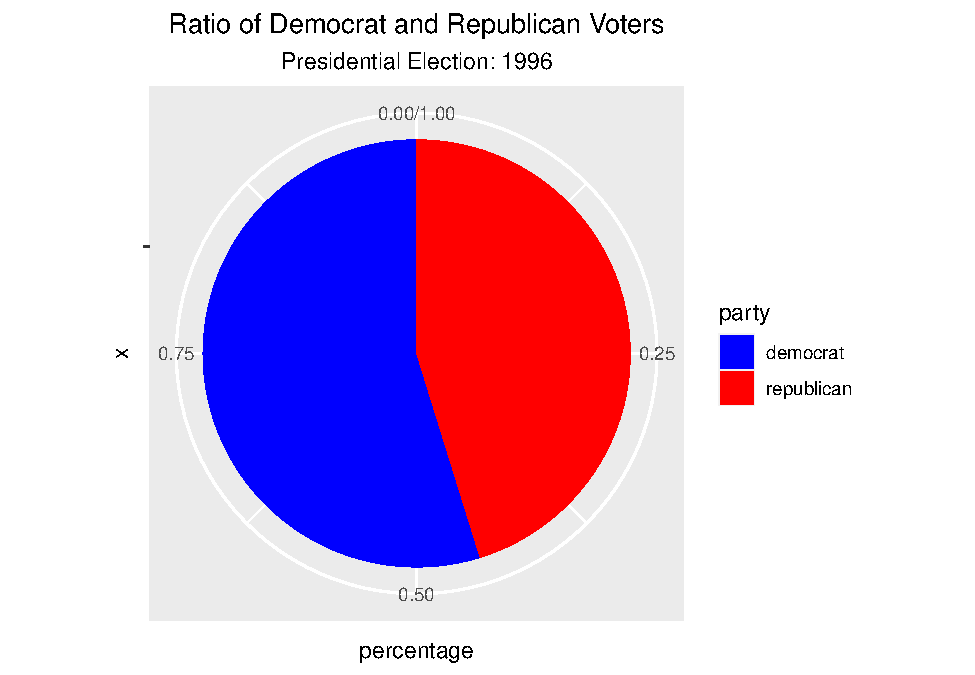
\includegraphics{election_files/figure-latex/anim-47.pdf}
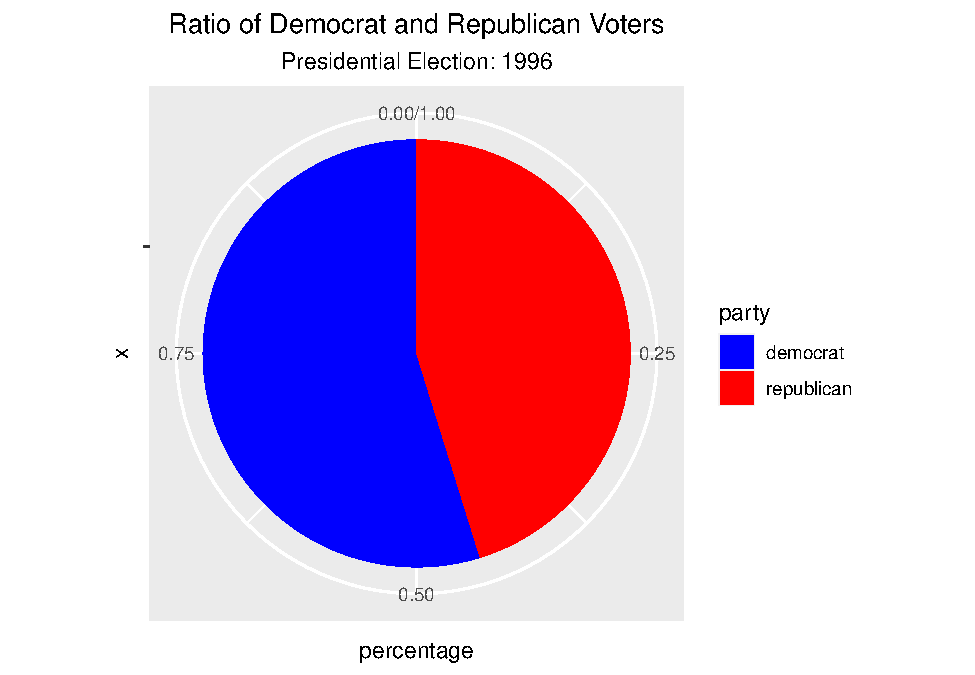
\includegraphics{election_files/figure-latex/anim-48.pdf}
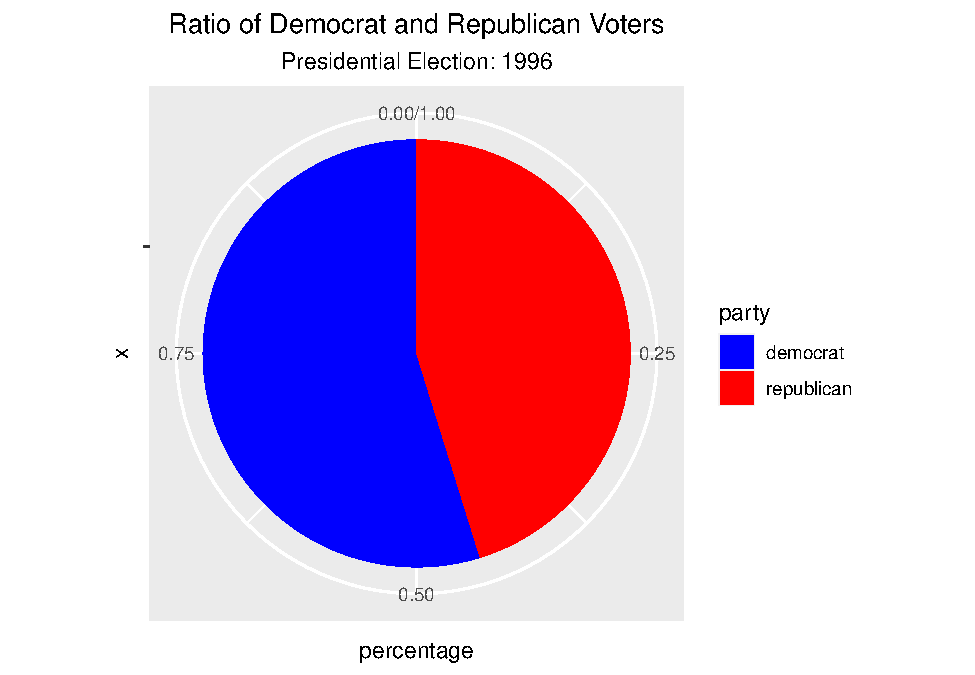
\includegraphics{election_files/figure-latex/anim-49.pdf}
\includegraphics{election_files/figure-latex/anim-50.pdf}
\includegraphics{election_files/figure-latex/anim-51.pdf}
\includegraphics{election_files/figure-latex/anim-52.pdf}
\includegraphics{election_files/figure-latex/anim-53.pdf}
\includegraphics{election_files/figure-latex/anim-54.pdf}
\includegraphics{election_files/figure-latex/anim-55.pdf}
\includegraphics{election_files/figure-latex/anim-56.pdf}
\includegraphics{election_files/figure-latex/anim-57.pdf}
\includegraphics{election_files/figure-latex/anim-58.pdf}
\includegraphics{election_files/figure-latex/anim-59.pdf}
\includegraphics{election_files/figure-latex/anim-60.pdf}
\includegraphics{election_files/figure-latex/anim-61.pdf}
\includegraphics{election_files/figure-latex/anim-62.pdf}
\includegraphics{election_files/figure-latex/anim-63.pdf}
\includegraphics{election_files/figure-latex/anim-64.pdf}
\includegraphics{election_files/figure-latex/anim-65.pdf}
\includegraphics{election_files/figure-latex/anim-66.pdf}
\includegraphics{election_files/figure-latex/anim-67.pdf}
\includegraphics{election_files/figure-latex/anim-68.pdf}
\includegraphics{election_files/figure-latex/anim-69.pdf}
\includegraphics{election_files/figure-latex/anim-70.pdf}
\includegraphics{election_files/figure-latex/anim-71.pdf}
\includegraphics{election_files/figure-latex/anim-72.pdf}
\includegraphics{election_files/figure-latex/anim-73.pdf}
\includegraphics{election_files/figure-latex/anim-74.pdf}
\includegraphics{election_files/figure-latex/anim-75.pdf}
\includegraphics{election_files/figure-latex/anim-76.pdf}
\includegraphics{election_files/figure-latex/anim-77.pdf}
\includegraphics{election_files/figure-latex/anim-78.pdf}
\includegraphics{election_files/figure-latex/anim-79.pdf}
\includegraphics{election_files/figure-latex/anim-80.pdf}
\includegraphics{election_files/figure-latex/anim-81.pdf}
\includegraphics{election_files/figure-latex/anim-82.pdf}
\includegraphics{election_files/figure-latex/anim-83.pdf}
\includegraphics{election_files/figure-latex/anim-84.pdf}
\includegraphics{election_files/figure-latex/anim-85.pdf}
\includegraphics{election_files/figure-latex/anim-86.pdf}
\includegraphics{election_files/figure-latex/anim-87.pdf}
\includegraphics{election_files/figure-latex/anim-88.pdf}
\includegraphics{election_files/figure-latex/anim-89.pdf}
\includegraphics{election_files/figure-latex/anim-90.pdf}
\includegraphics{election_files/figure-latex/anim-91.pdf}
\includegraphics{election_files/figure-latex/anim-92.pdf}
\includegraphics{election_files/figure-latex/anim-93.pdf}
\includegraphics{election_files/figure-latex/anim-94.pdf}
\includegraphics{election_files/figure-latex/anim-95.pdf}
\includegraphics{election_files/figure-latex/anim-96.pdf}
\includegraphics{election_files/figure-latex/anim-97.pdf}
\includegraphics{election_files/figure-latex/anim-98.pdf}
\includegraphics{election_files/figure-latex/anim-99.pdf}
\includegraphics{election_files/figure-latex/anim-100.pdf}

\hypertarget{bibliography}{%
\subsection{Bibliography}\label{bibliography}}

\begin{verbatim}
Data
- author    : MIT Election Data and Science Lab,
- publisher : Harvard Dataverse,
- title     : U.S. President 1976–2016,
- UNF       : UNF:6:Mw0hOUHAijKPTVRAe5jJvg==,
- year      : 2017,
- version   : V5,
- doi       : 10.7910/DVN/42MVDX,
- url       : https://doi.org/10.7910/DVN/42MVDX
\end{verbatim}

\end{document}
